\subsection{Vortex Induced Vibration}
Vortex Induced Vibrations (VIV) are motions of solid structures immersed in fluid that is caused by the irregularities in the flow. VIV of structures is of practical interest to many fields of engineering. For example, it can cause vibration and noise in heat exchanger tubes and an aircraft wing. The practical significance of VIV has led to various studies discussed in the literature\cite{williamson2004vortex}. In this demonstration problem, we are interested in the forced oscillations of an elastically mounted, rigid cylinder for different values of the Reynolds number. The physical problem is shown in Figure \ref{fig:C5_cylinderShape}.
%
\begin{figure}[H]
    \centering
    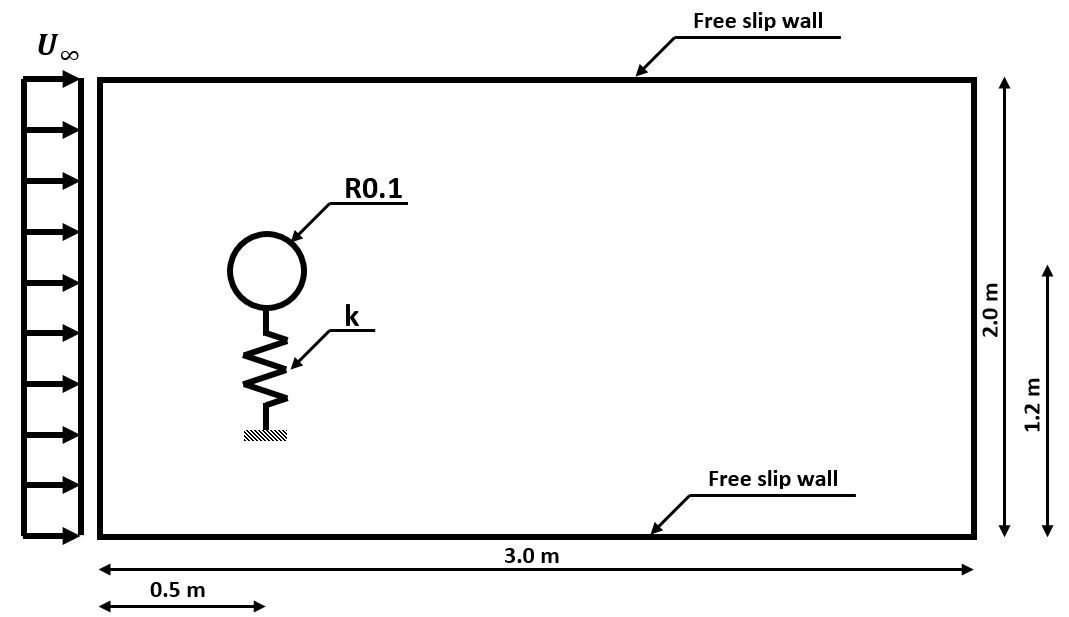
\includegraphics[width=9.00cm]{Chapter_5/figure/VIV_domain_shape.jpg}
    \caption{Physical domain for the vortex induced vibration problem.}
    \label{fig:C5_cylinderShape}
\end{figure}
%
The rigid cylinder has the radius $R$ and is mounted on an elastic structure with stiffness $k$. The free steam velocity is selected as $U_\infty$. To verify the solver and FSI coupling, we are going to calculate the shedding frequency of the cylinder first. Vortex shedding is an oscillating flow that takes place when fluid passes a bluff body at certain velocities. The vortices that are generated on the aft of the body start to detach periodically from either side of the body. The frequency at which the vortex shedding takes place is described using the dimensionless Strouhal number. The Strouhal number is defined as shown in Equation \eqref{eq:C5_strouhalNumber}.
%
\begin{equation}\label{eq:C5_strouhalNumber}
	St = \frac{fL}{U}
\end{equation}
%
where $f$ is the frequency of the vortex shedding; $L$ is the characteristic length; and $U$ is the flow velocity. The Strouhal number of a stationary circular cylinder is a function of Reynolds number \cite{chen1987flow} as shown in Figure \ref{fig:C5_strouhalVSreynoldsNumber}\cite{jendrzejczyk1985fluid}.
%
\begin{figure}[H]
    \centering
    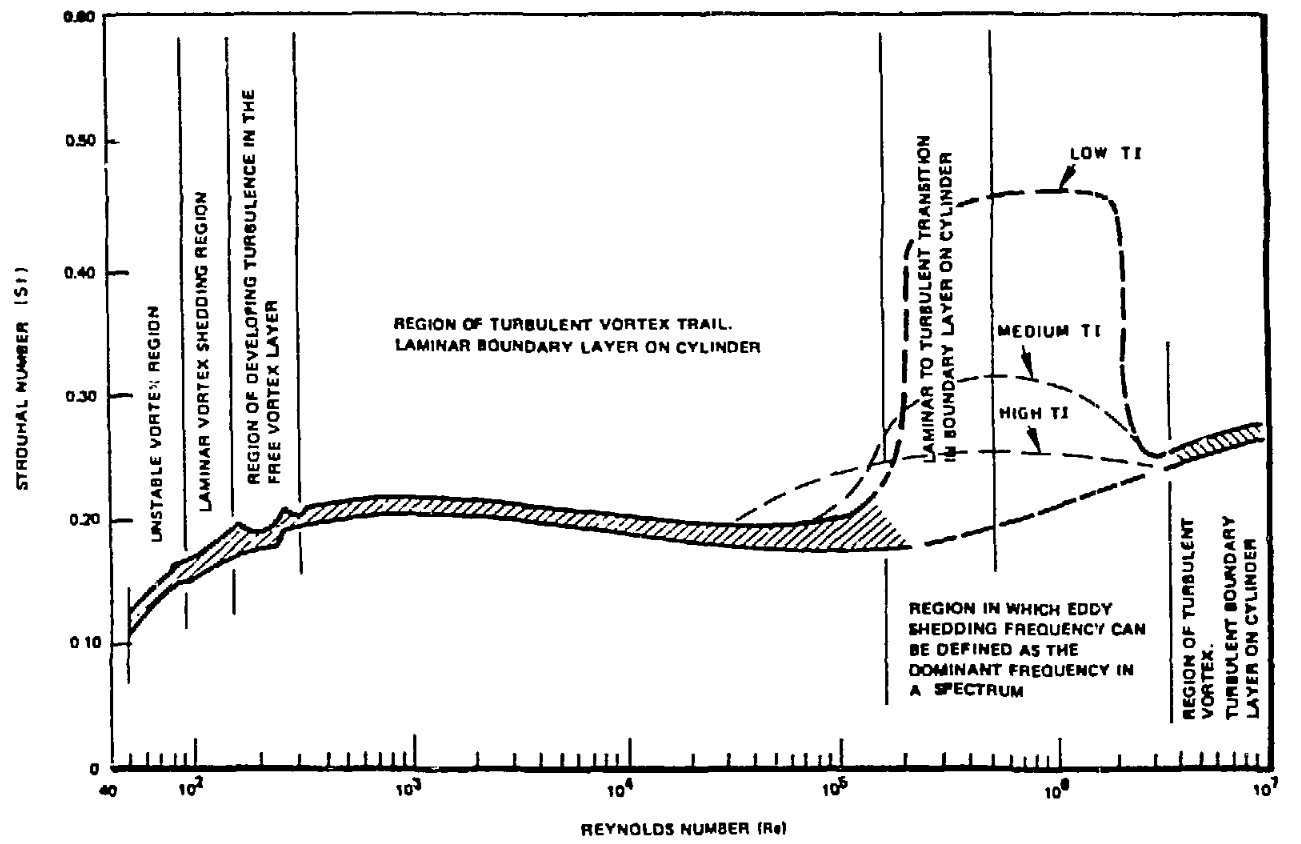
\includegraphics[width=10.00cm]{Chapter_5/figure/StrouhalVsReynodsl.png}
    \caption{Strouhal number for a single cylinder.}
    \label{fig:C5_strouhalVSreynoldsNumber}
\end{figure}
%
To verify the simulation code developed for the IB simulation, we verified the shedding frequency of the circular cylinder in the cross-flow. The domain length and height are selected as $3 m$ and $2 m$, respectively, as shown in Figure \ref{fig:C5_cylinderShape}. The cylinder radius is selected as $0.1 m$ and is located $0.5 m$ from the left wall and $1.2 m$ from the bottom wall. The asymmetric shape of the computational domain helps the shedding initiation. The domain is discretized using $3000$ cells in the $x$ and $2000$ in the $y$ direction. The cylinder is defined using $50$ Lagrangian nodes. The $p$ value in the delta function definition is selected as $0.5$. It should be noted that to verify the shedding frequency the cylinder is fixed in its place. We compared the Strouhal number calculated from the IB code with the results \cite{mittal2001control} for two different Reynolds numbers. The shedding frequency is calculated by saving the time history of drag force on the cylinder and performing frequency analysis on this data. We used the power spectral density function to look at the most dominant frequencies. The comparison between these results is shown in Table \ref{table:C5_strouhalVerification}.
%
\begin{table}[H]
\centering
\begin{tabular}{c | c | c}
     Reynolds number & St (current IB) & St (Literature \cite{jendrzejczyk1985fluid} and \cite{mittal2001control}) \\ \hline \hline
     100 & 0.171 & 0.168 \\ \hline
     500 & 0.194 & 0.200 \\
\end{tabular}
\caption{Comparison between the shedding frequency calcualted using IB method and results from the literature.}
\label{table:C5_strouhalVerification}
\end{table}
%
The effect of the number of Lagrangian points on the shedding frequency is shown in Figure \ref{fig:C5_numberOfLagrangianOnSheddingFreq} for the two Reynolds numbers of 100 and 500. As shown here, the number of Lagrangian points does not affect the vortex shedding frequency.
%
\begin{figure}[H]
    \centering
    \subfigure[$Re = 100$]
    {
    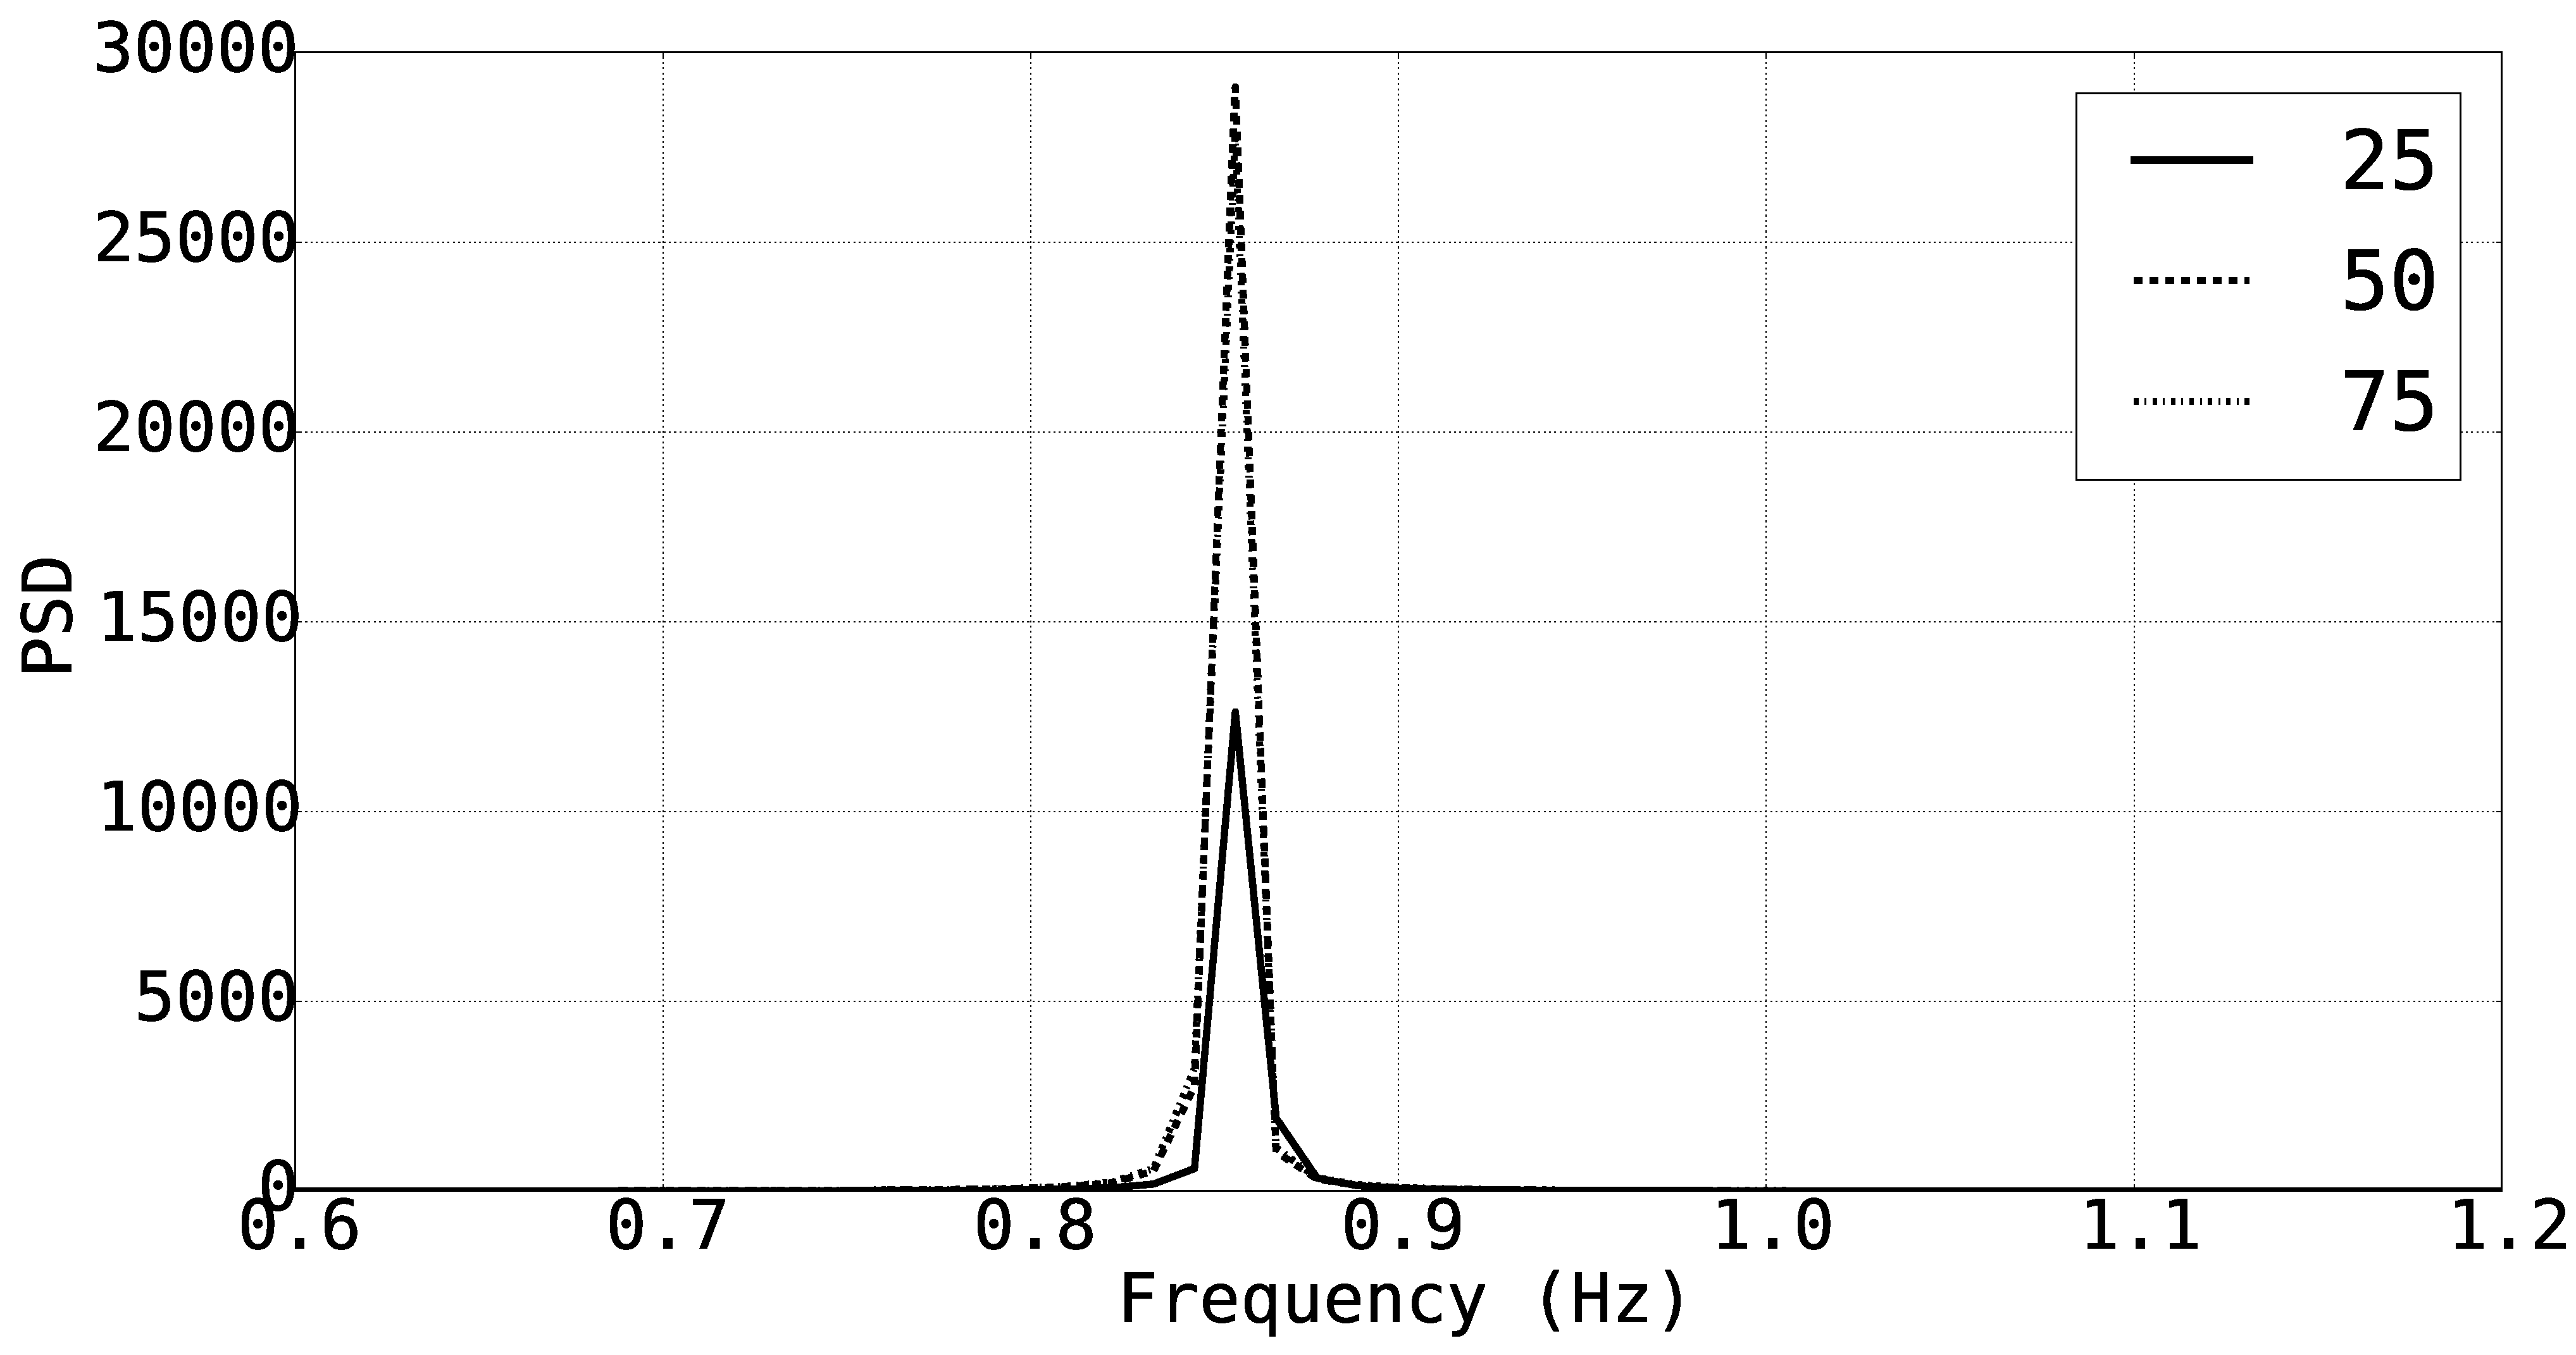
\includegraphics[width=9.0cm]{Chapter_5/figure/PSD_Re100.eps}
    }
    \quad
    \subfigure[$Re = 500$]
    {
    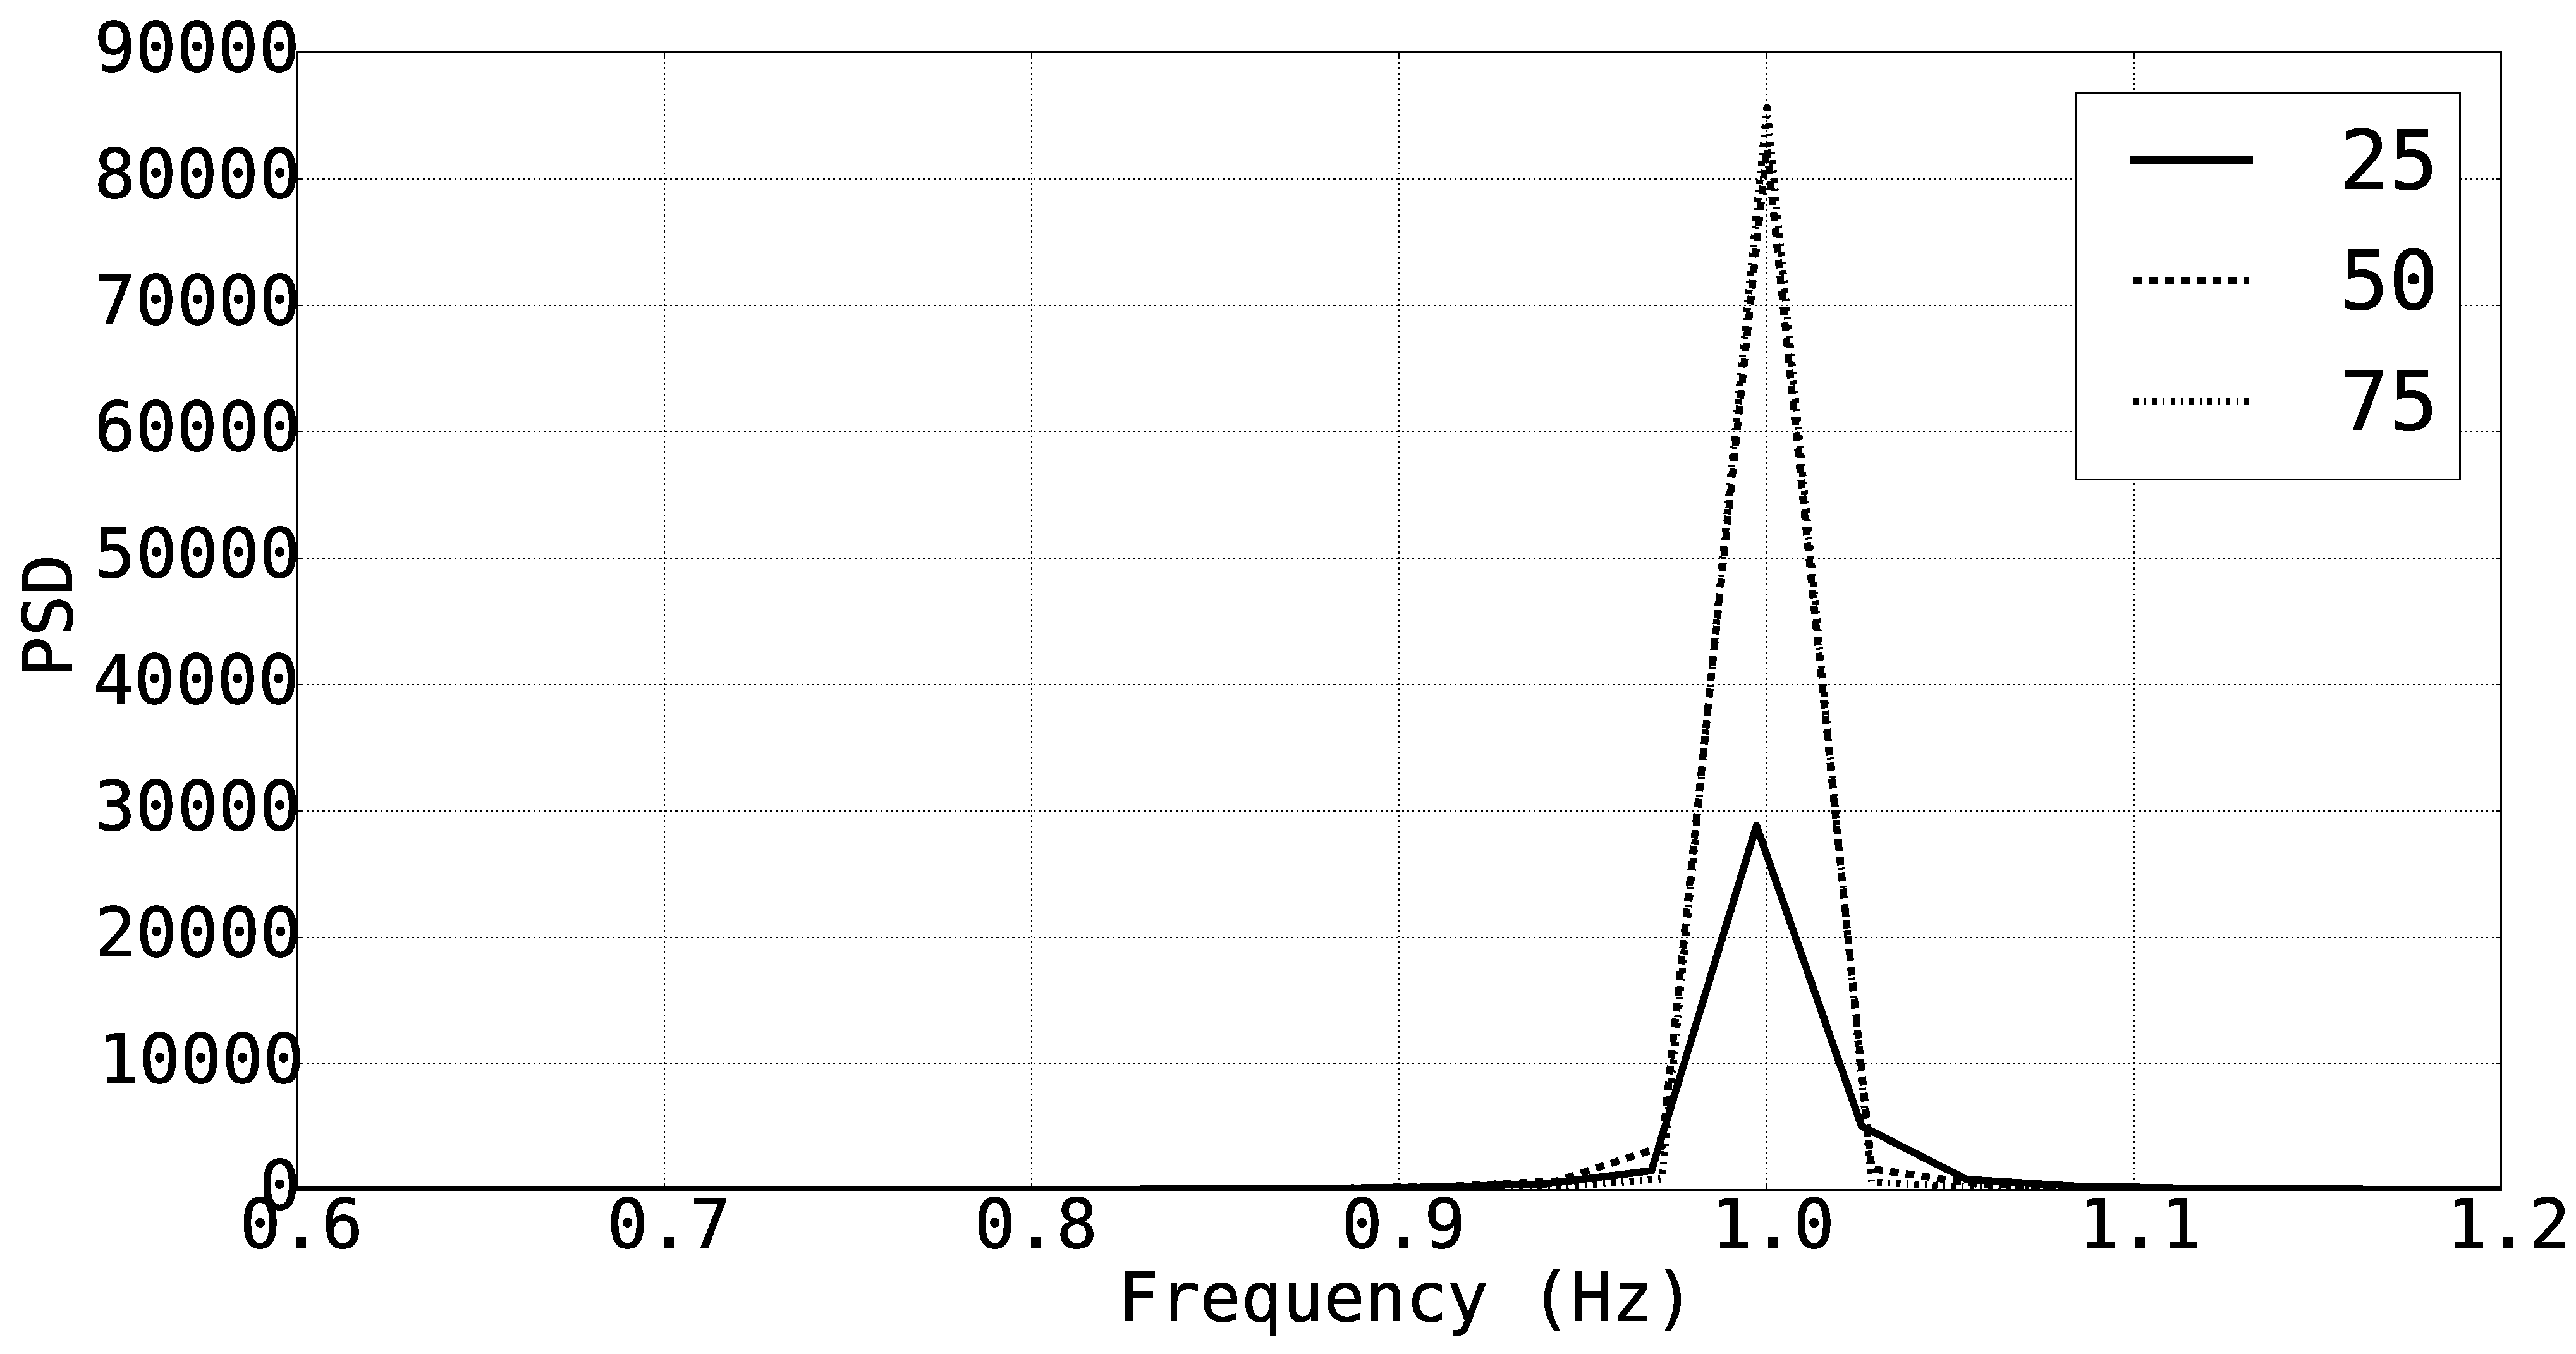
\includegraphics[width=9.0cm]{Chapter_5/figure/PSD_Re500.eps}
    }
    \caption{Number of Lagrangian points effect on the shedding frequency.}
    \label{fig:C5_numberOfLagrangianOnSheddingFreq}
\end{figure}
%
After verifying the shedding frequency of IB solver, we attach the elastic structure to the cylinder and let the system vibrate due to aerodynamic loads. The equation of motion for this cylinder is shown in Equation \eqref{eq:C5_cylinderEquationOfMotion}.
%
\begin{equation}\label{eq:C5_cylinderEquationOfMotion}
	m \ddot{y} + k y = f(y, \dot{y}, t; R)
\end{equation}
%
where $y$ is the cylinder location; $m$ is the cylinder mass; $k$ is elastic structure stiffness; and $f(y, \dot{y}, t; R)$ is the aerodynamic load. It should be noted that the load is an explicit function of cylinder location, velocity, time, and an implicit function of cylinder radius. This requires an unsteady treatment of the FSI problem by coupling Equation \eqref{eq:C5_fluidGE} and \eqref{eq:C5_cylinderEquationOfMotion}.

At each time step, the NS equations are solved and the pressure values at the Lagrangian nodes are calculated using the regularized Delta function. These pressure values are then integrated over the cylinder surface to calculate the force value on the right-hand-side of Equation \eqref{eq:C5_cylinderEquationOfMotion}. To solve for the structure displacement and velocity, Equation \eqref{eq:C5_cylinderEquationOfMotion} is written in the state-space form as shown in Equation \eqref{eq:C5_cylinderEquationOfMotionStateSpace}. This equation is then integrated in time alongside the NS equations using Adams-bashforth method. The initial condition for the structure is selected as zero displacement and velocity at $t = 0$.
%
\begin{equation}\label{eq:C5_cylinderEquationOfMotionStateSpace}
	\begin{bmatrix}
	\dot{y} \\
	\ddot{y}
	\end{bmatrix} = 
	\begin{bmatrix}
	0 & 1 \\
	-\dfrac{k}{m} & 0
	\end{bmatrix}
	\begin{bmatrix}
	y \\
	\dot{y}
	\end{bmatrix} + 
	\begin{bmatrix}
	0 \\
	f(y, \dot{y}, t; R)
	\end{bmatrix}
\end{equation}
%
where the load, $f(y, \dot{y}, t; R)$, is calculated  as shown in Equation \eqref{eq:C5_loadOnCylidner}.
%
\begin{equation}\label{eq:C5_loadOnCylidner}
	f = \oint \left( \int \int p(x, y) \mathcal{D}(x - X_s) \mathcal{D}(y - Y_s) dx dy\right) ds
\end{equation}
%
In Equation \eqref{eq:C5_loadOnCylidner}, $p(x, y)$ is the pressure calculated from the CFD solution; $\mathcal{D}$ is the regularized delta function; and $ds$ represents the infinitesimal element on the cylinder surface.

For the coupled FSI sensitivity analysis, we looked at the vortex induced vibration of the cylinder at two different Reynolds numbers. The sensitivity of the displacement to the radius of the cylinder is calculated and verified with the complex step results. The sensitivity equations for the fluid domain is derived in Chapter \ref{ch:shapeSenwithIB} and by solving it we have the sensitivity of pressure field on the surface of the cylinder. The sensitivity equation for the structure is derived by differentiating Equation \eqref{eq:C5_cylinderEquationOfMotionStateSpace} as shown in Equation \eqref{eq:C5_cylinderEquationOfMotionSAStateSpace}.
%
\begin{equation}\label{eq:C5_cylinderEquationOfMotionSAStateSpace}
	\begin{bmatrix}
	\dot{y'} \\
	\ddot{y'}
	\end{bmatrix} = 
	\begin{bmatrix}
	0 & 1 \\
	-\dfrac{k}{m} & 0
	\end{bmatrix}
	\begin{bmatrix}
	y' \\
	\dot{y'}
	\end{bmatrix} + 
	\begin{bmatrix}
	0 \\
	f'(y, \dot{y}, t; R)
	\end{bmatrix}
\end{equation}
%
here, $()'$, represents the derivative with respect to the design variable. As can be seen the same solver used for solving Equation \eqref{eq:C5_cylinderEquationOfMotionStateSpace} is utilized for solving Equation \eqref{eq:C5_cylinderEquationOfMotionSAStateSpace}. The only difference between the two is the loads used for evaluating the right-hand-side of Equation \eqref{eq:C5_cylinderEquationOfMotionSAStateSpace}.

For this problem, the stiffness of the elastic structure, $k$, is selected as 1 N/m and the cylinder mass is chosen as 1 kg. The time history of cylinder displacement in the first 25 seconds of its motion is shown in Figure \ref{fig:C5_cylinderDisplacement}. As can be seen here, the cylinder starts from the initial position at $y=1.2$ and after a short transient region starts oscillating at an almost constant amplitude. As shown in Figure \ref{fig:C5_cylinderDisplacement}.
%
\begin{figure}[H]
    \centering
    \subfigure[$Re = 100$]
    {
    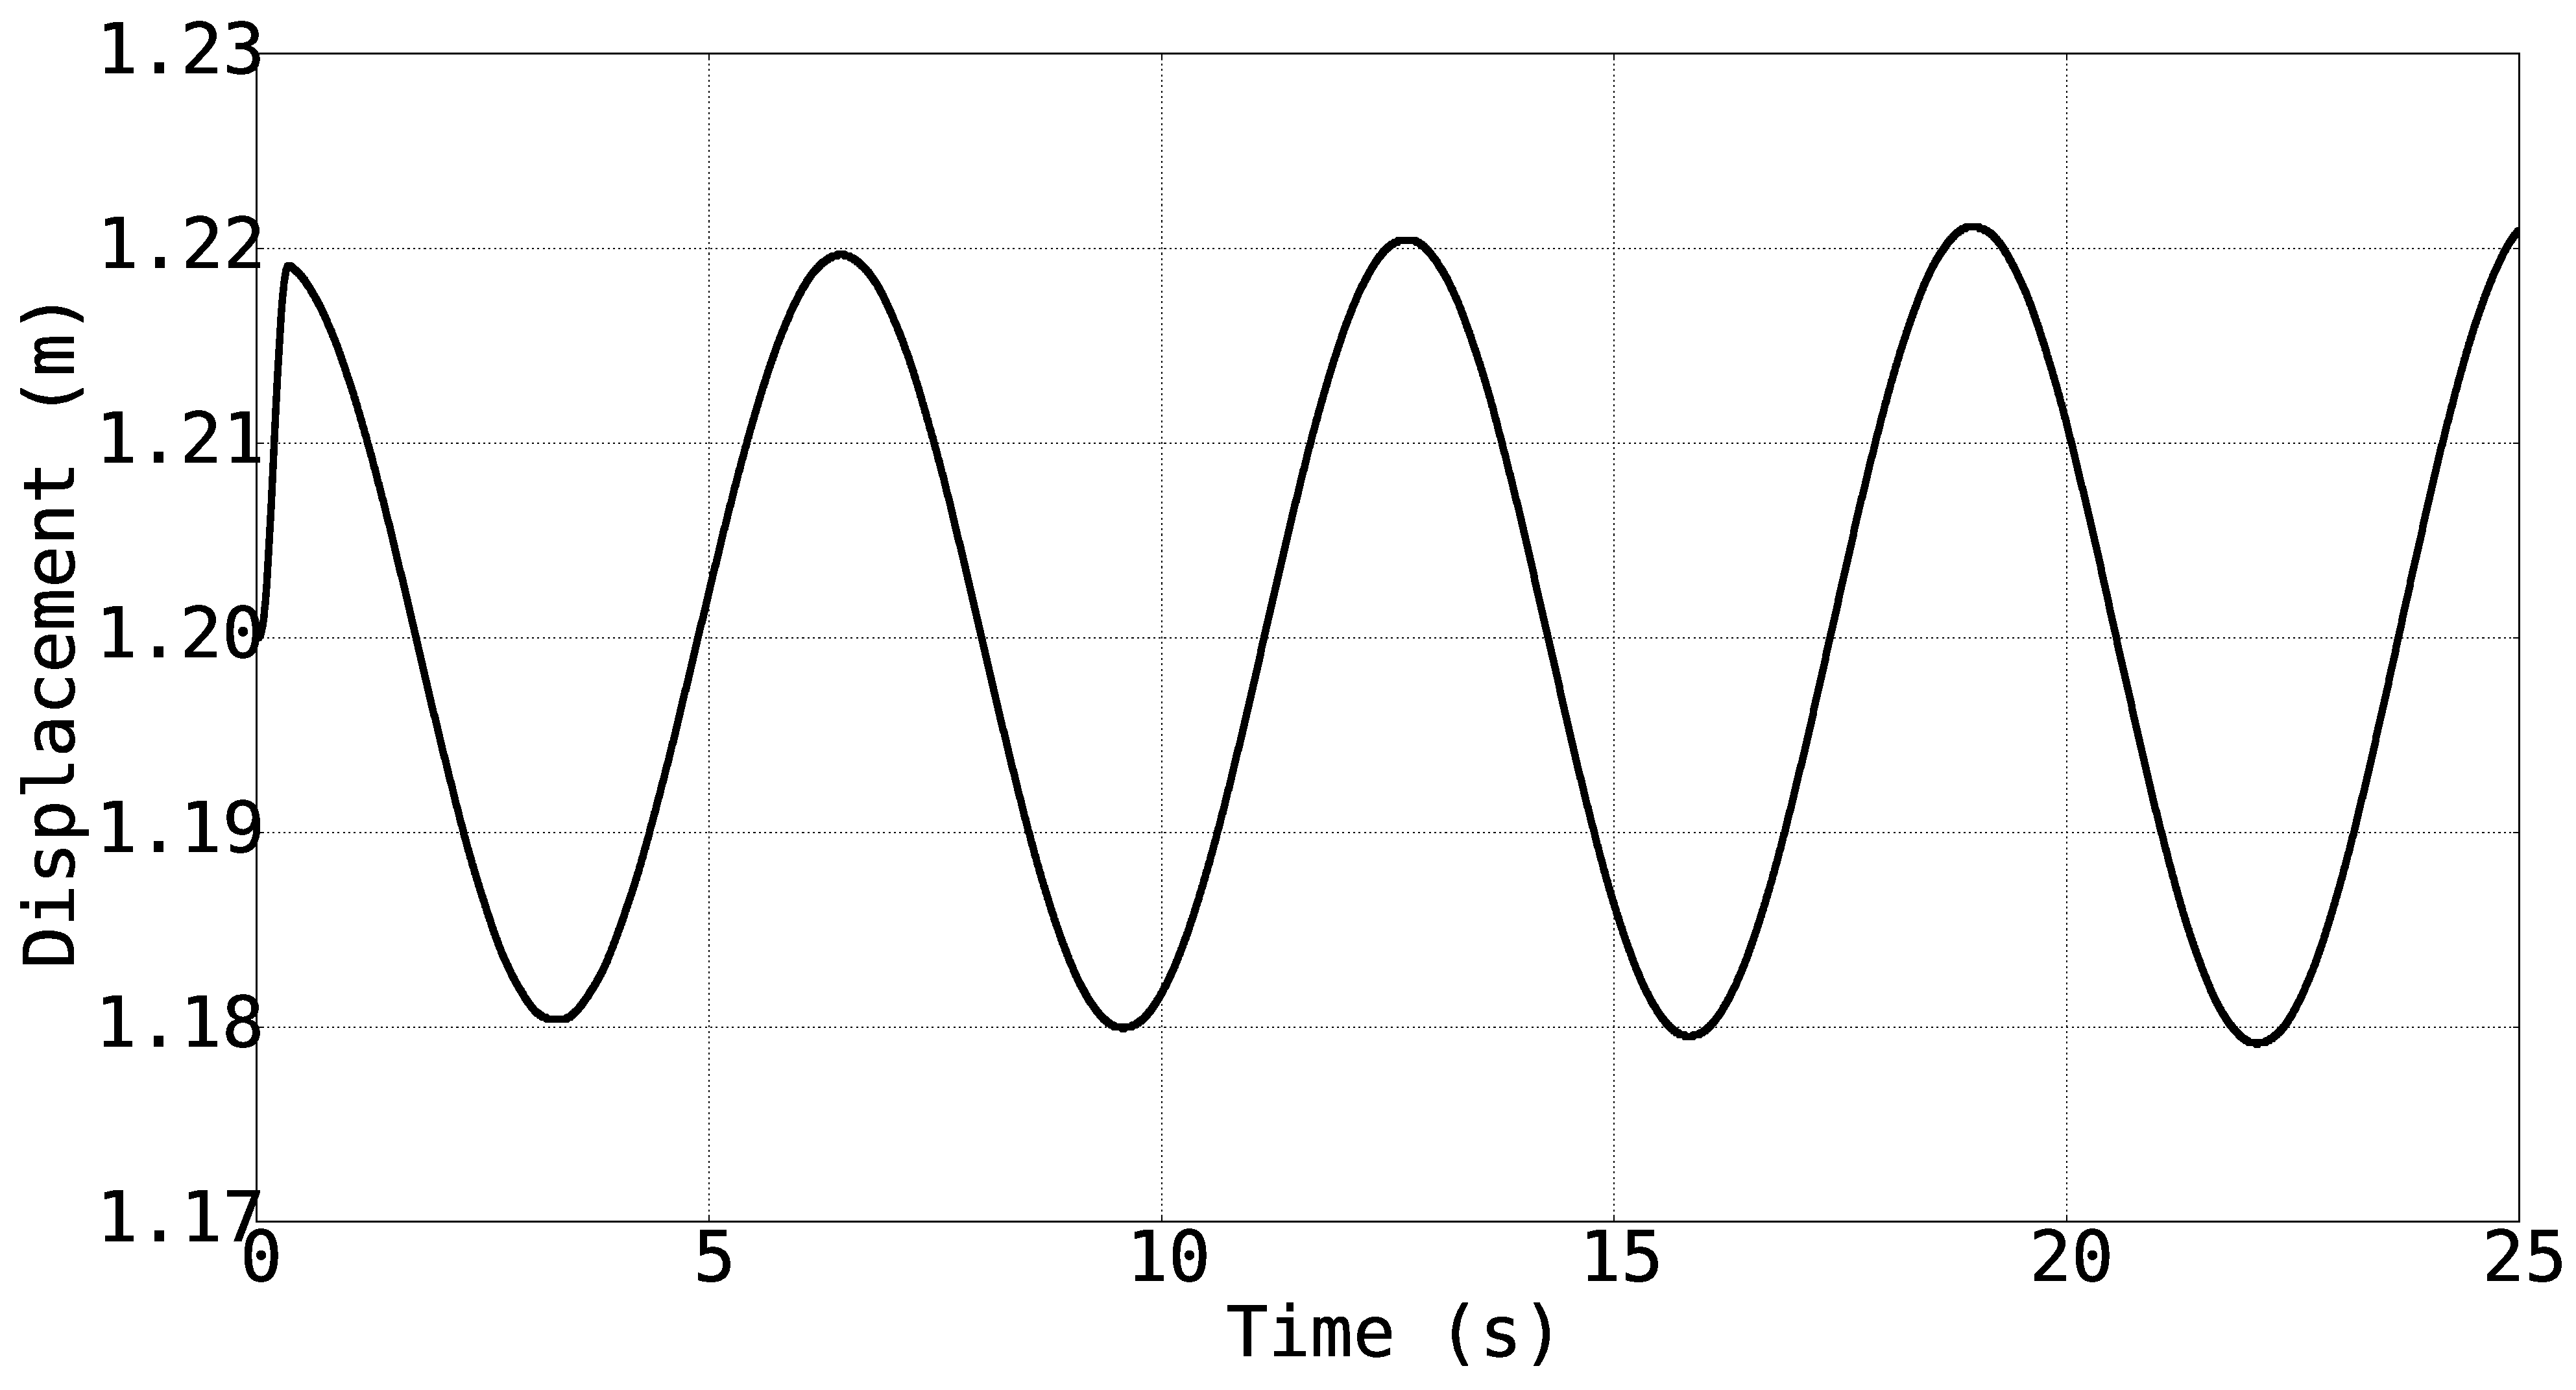
\includegraphics[width=9.0cm]{Chapter_5/figure/cylinder_Re100_Displacement.eps}
    }
    \quad
    \subfigure[$Re = 500$]
    {
    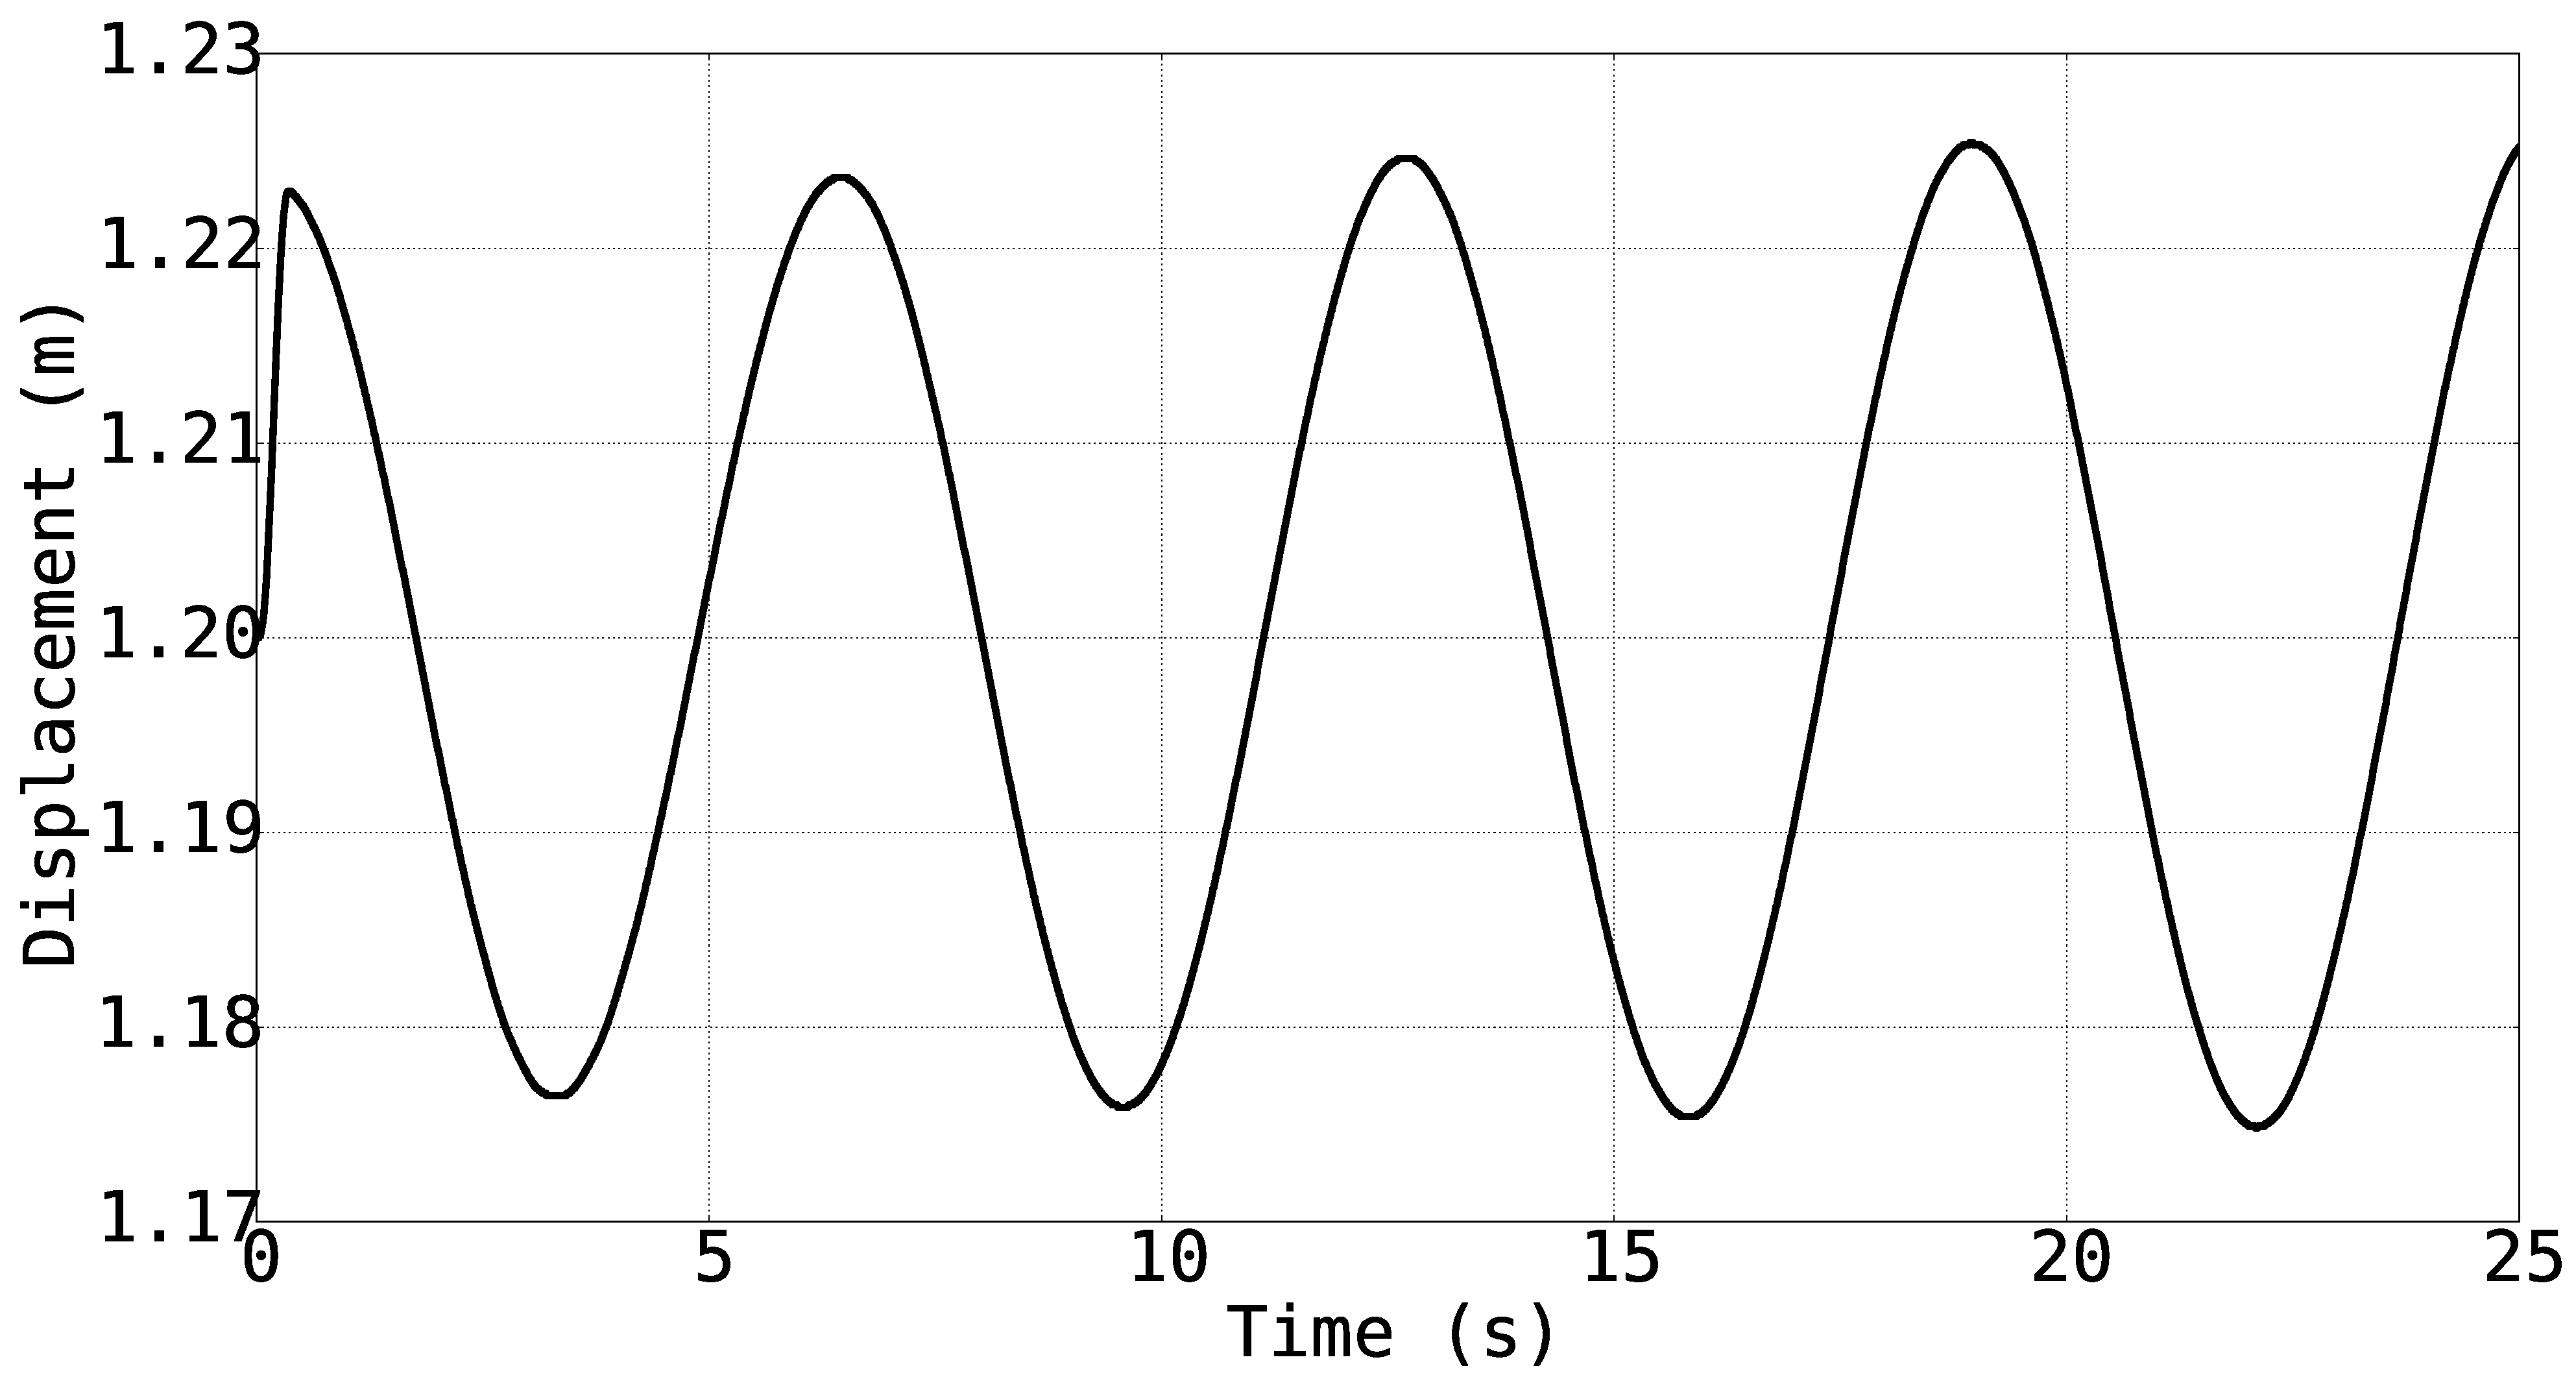
\includegraphics[width=9.0cm]{Chapter_5/figure/cylinder_Re500_Displacement.eps}
    }
    \caption{Time history of cylinder center displacement.}
    \label{fig:C5_cylinderDisplacement}
\end{figure}
%
Figure \ref{fig:C5_cylinderFSIvelocity} shows the u-velocity contour around the elastically mounted cylinder at different times. As can be seen, the vortex shedding is dominant at $t=5$. It should be noted that the vortex shedding starts before $t=5$ and causes the cylinder to oscillate.
%
\begin{figure}[H]
    \centering
    \subfigure[$Re = 100, t = 0 \text{ sec}$]
    {
    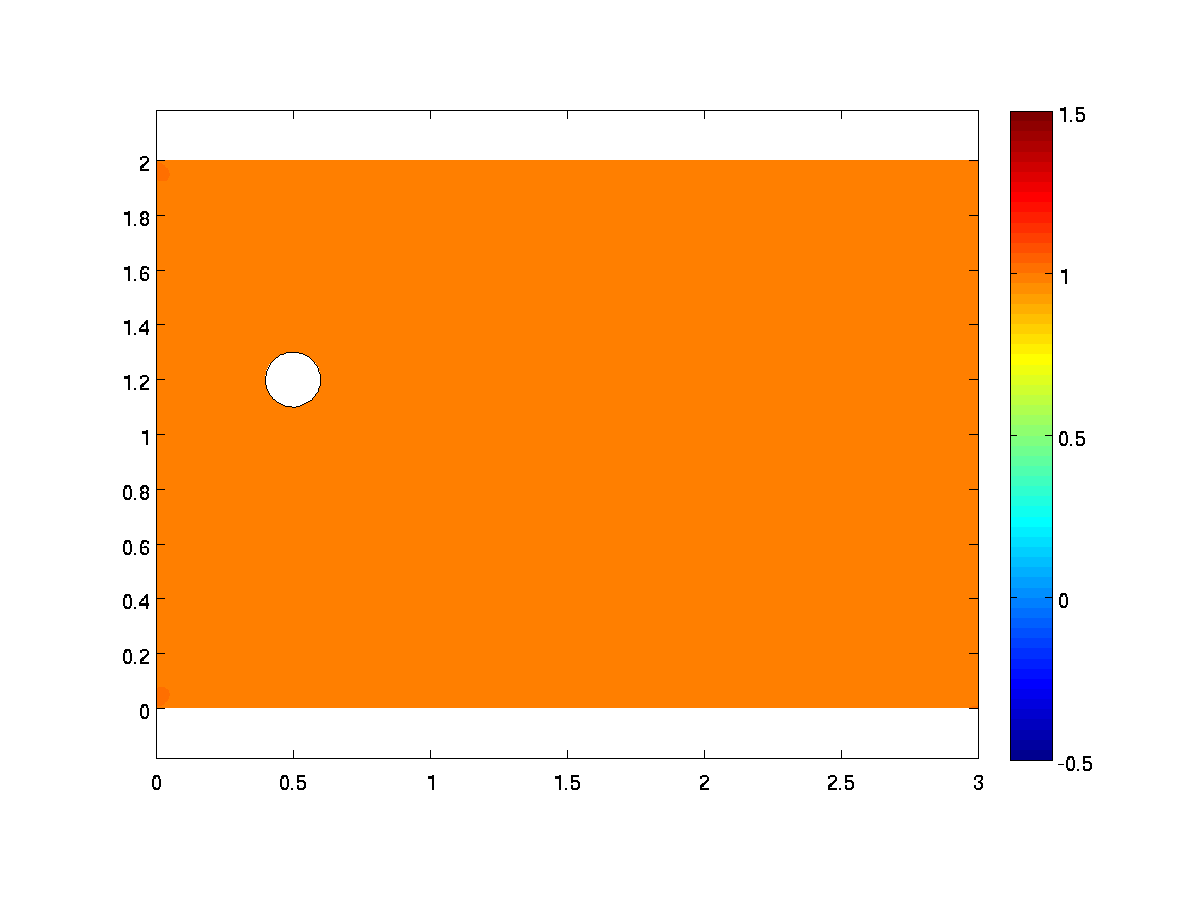
\includegraphics[width=6.0cm]{Chapter_5/figure/cylinder_analysis_Re100_t0.png}
    }
    \quad
    \subfigure[$Re = 500, t = 0 \text{ sec}$]
    {
    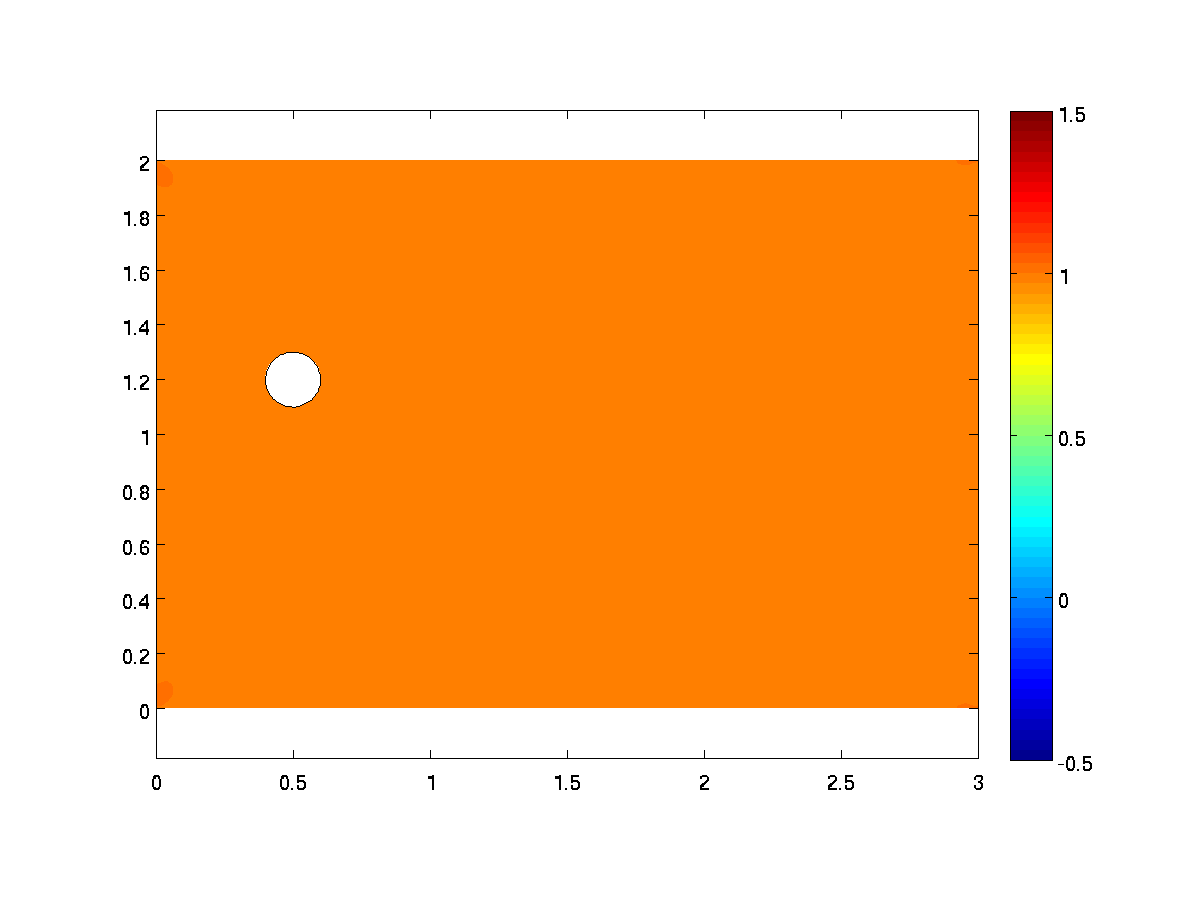
\includegraphics[width=6.0cm]{Chapter_5/figure/cylinder_analysis_Re500_t0.png}
    }
    \\
    \subfigure[$Re = 100, t = 0.5 \text{ ec}$]
    {
    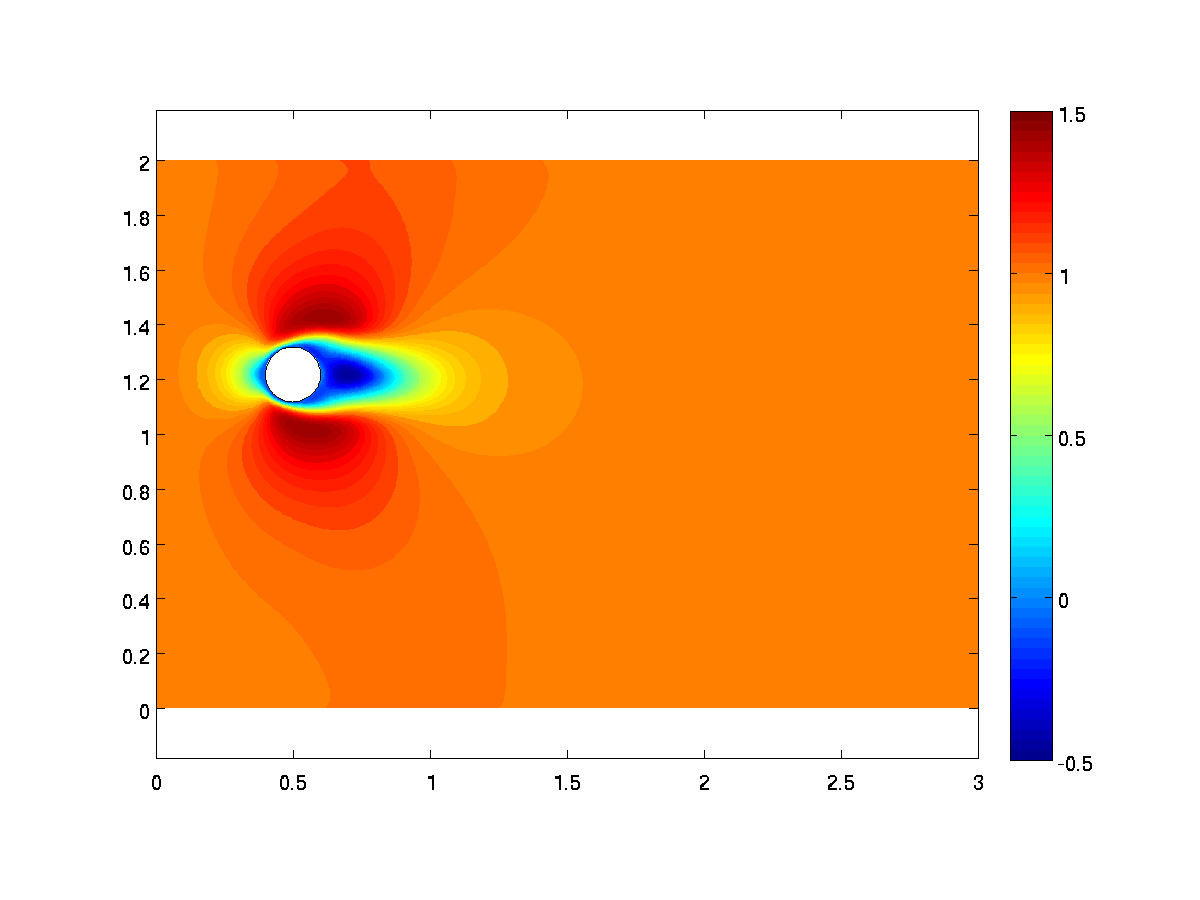
\includegraphics[width=6.0cm]{Chapter_5/figure/cylinder_analysis_Re100_t05.png}
    }
    \quad
    \subfigure[$Re = 500, t = 0.5 \text{ sec}$]
    {
    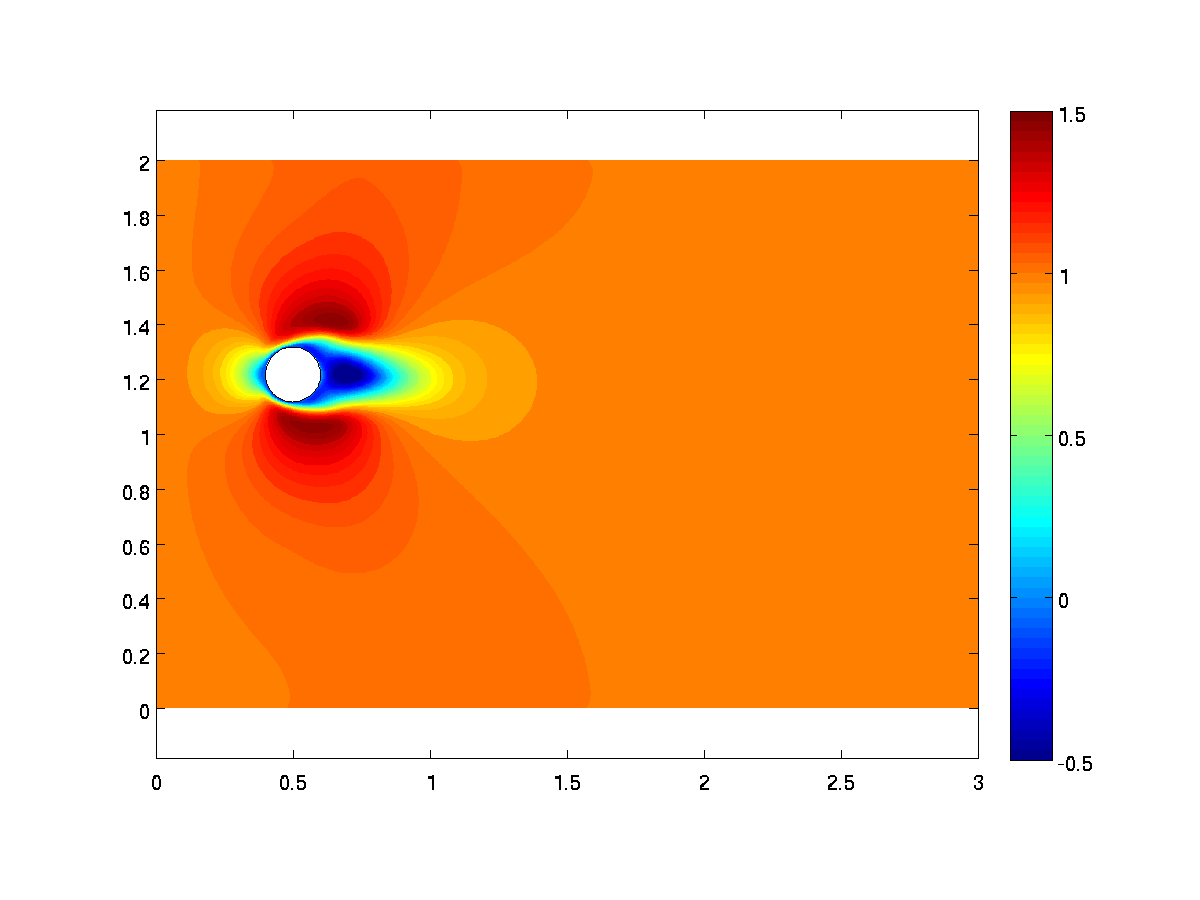
\includegraphics[width=6.0cm]{Chapter_5/figure/cylinder_analysis_Re500_t05.png}
    }
    \\
    \subfigure[$Re = 100, t = 5 \text{ sec}$]
    {
    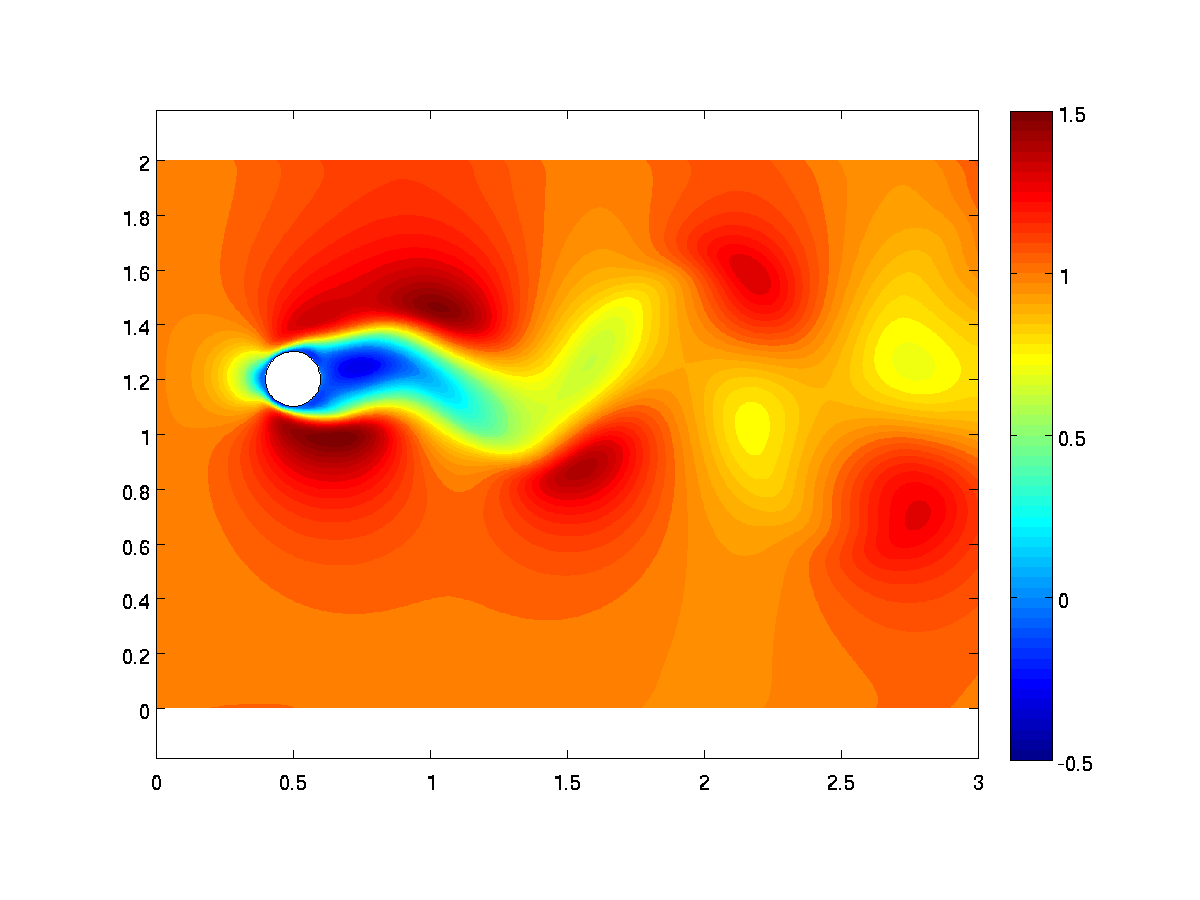
\includegraphics[width=6.0cm]{Chapter_5/figure/cylinder_analysis_Re100_t5.png}
    }
    \quad
    \subfigure[$Re = 500, t = 5 \text{ sec}$]
    {
    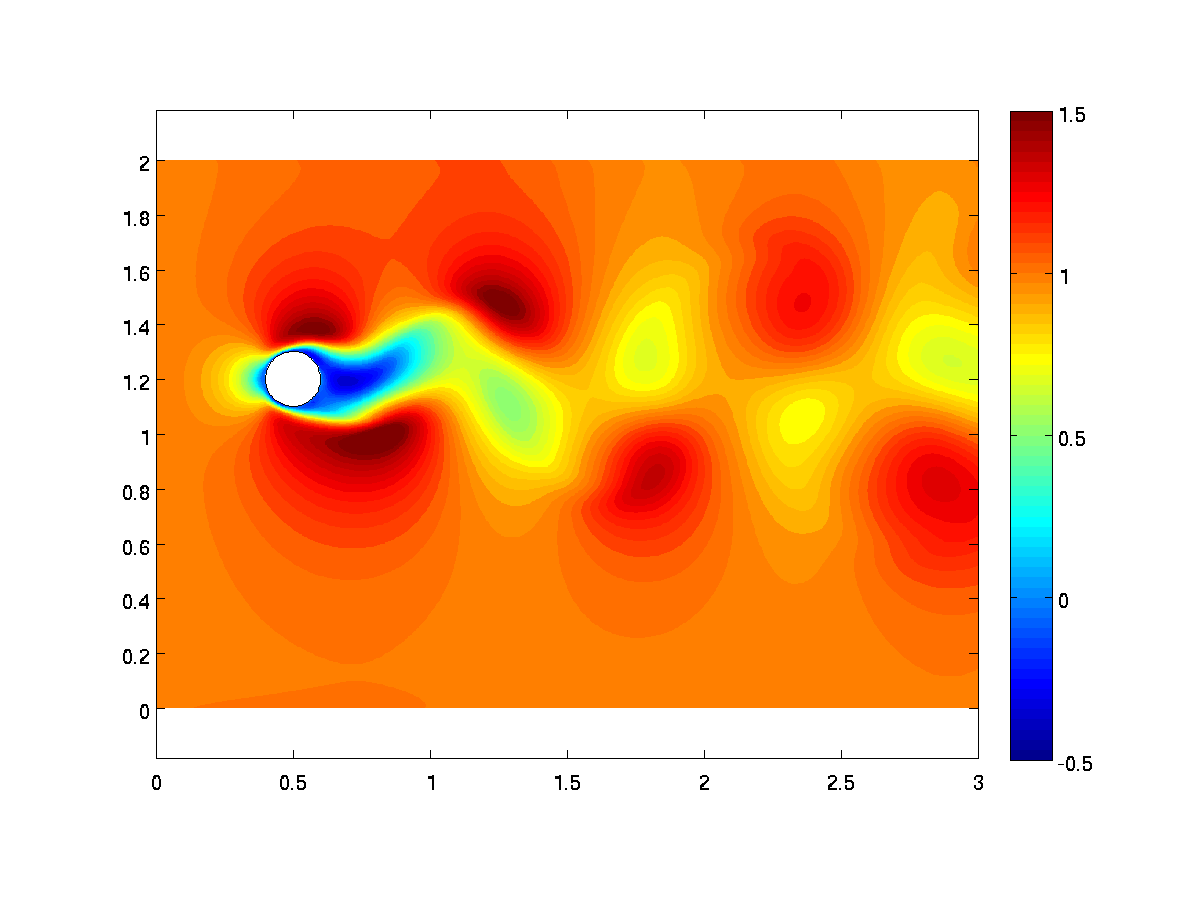
\includegraphics[width=6.0cm]{Chapter_5/figure/cylinder_analysis_Re500_t5.png}
    }
    \caption{Unsteady u-velocity contours for flow around cylinder at $Re = 100$ and $Re = 500$.}
    \label{fig:C5_cylinderFSIvelocity}
\end{figure}
%
The time history of the sensitivity results are shown and verified with the complex step solution in Figure \ref{fig:C5_cylinderDisplacementSensitivity}. As shown here, at the $t=0$ the sensitivity of displacement with respect to radius is zero since the cylinder at its initial location which is independent of its shape. However, the value of cylinder displacement will start oscillating between positive and negative numbers as the simulation continuous. This is what we are expecting since by increasing the radius, the loads on the cylinder will increase. This will result in increase in the amplitude in both ends of the oscillation period.
%
\begin{figure}[H]
    \centering
    \subfigure[$Re = 100$]
    {
    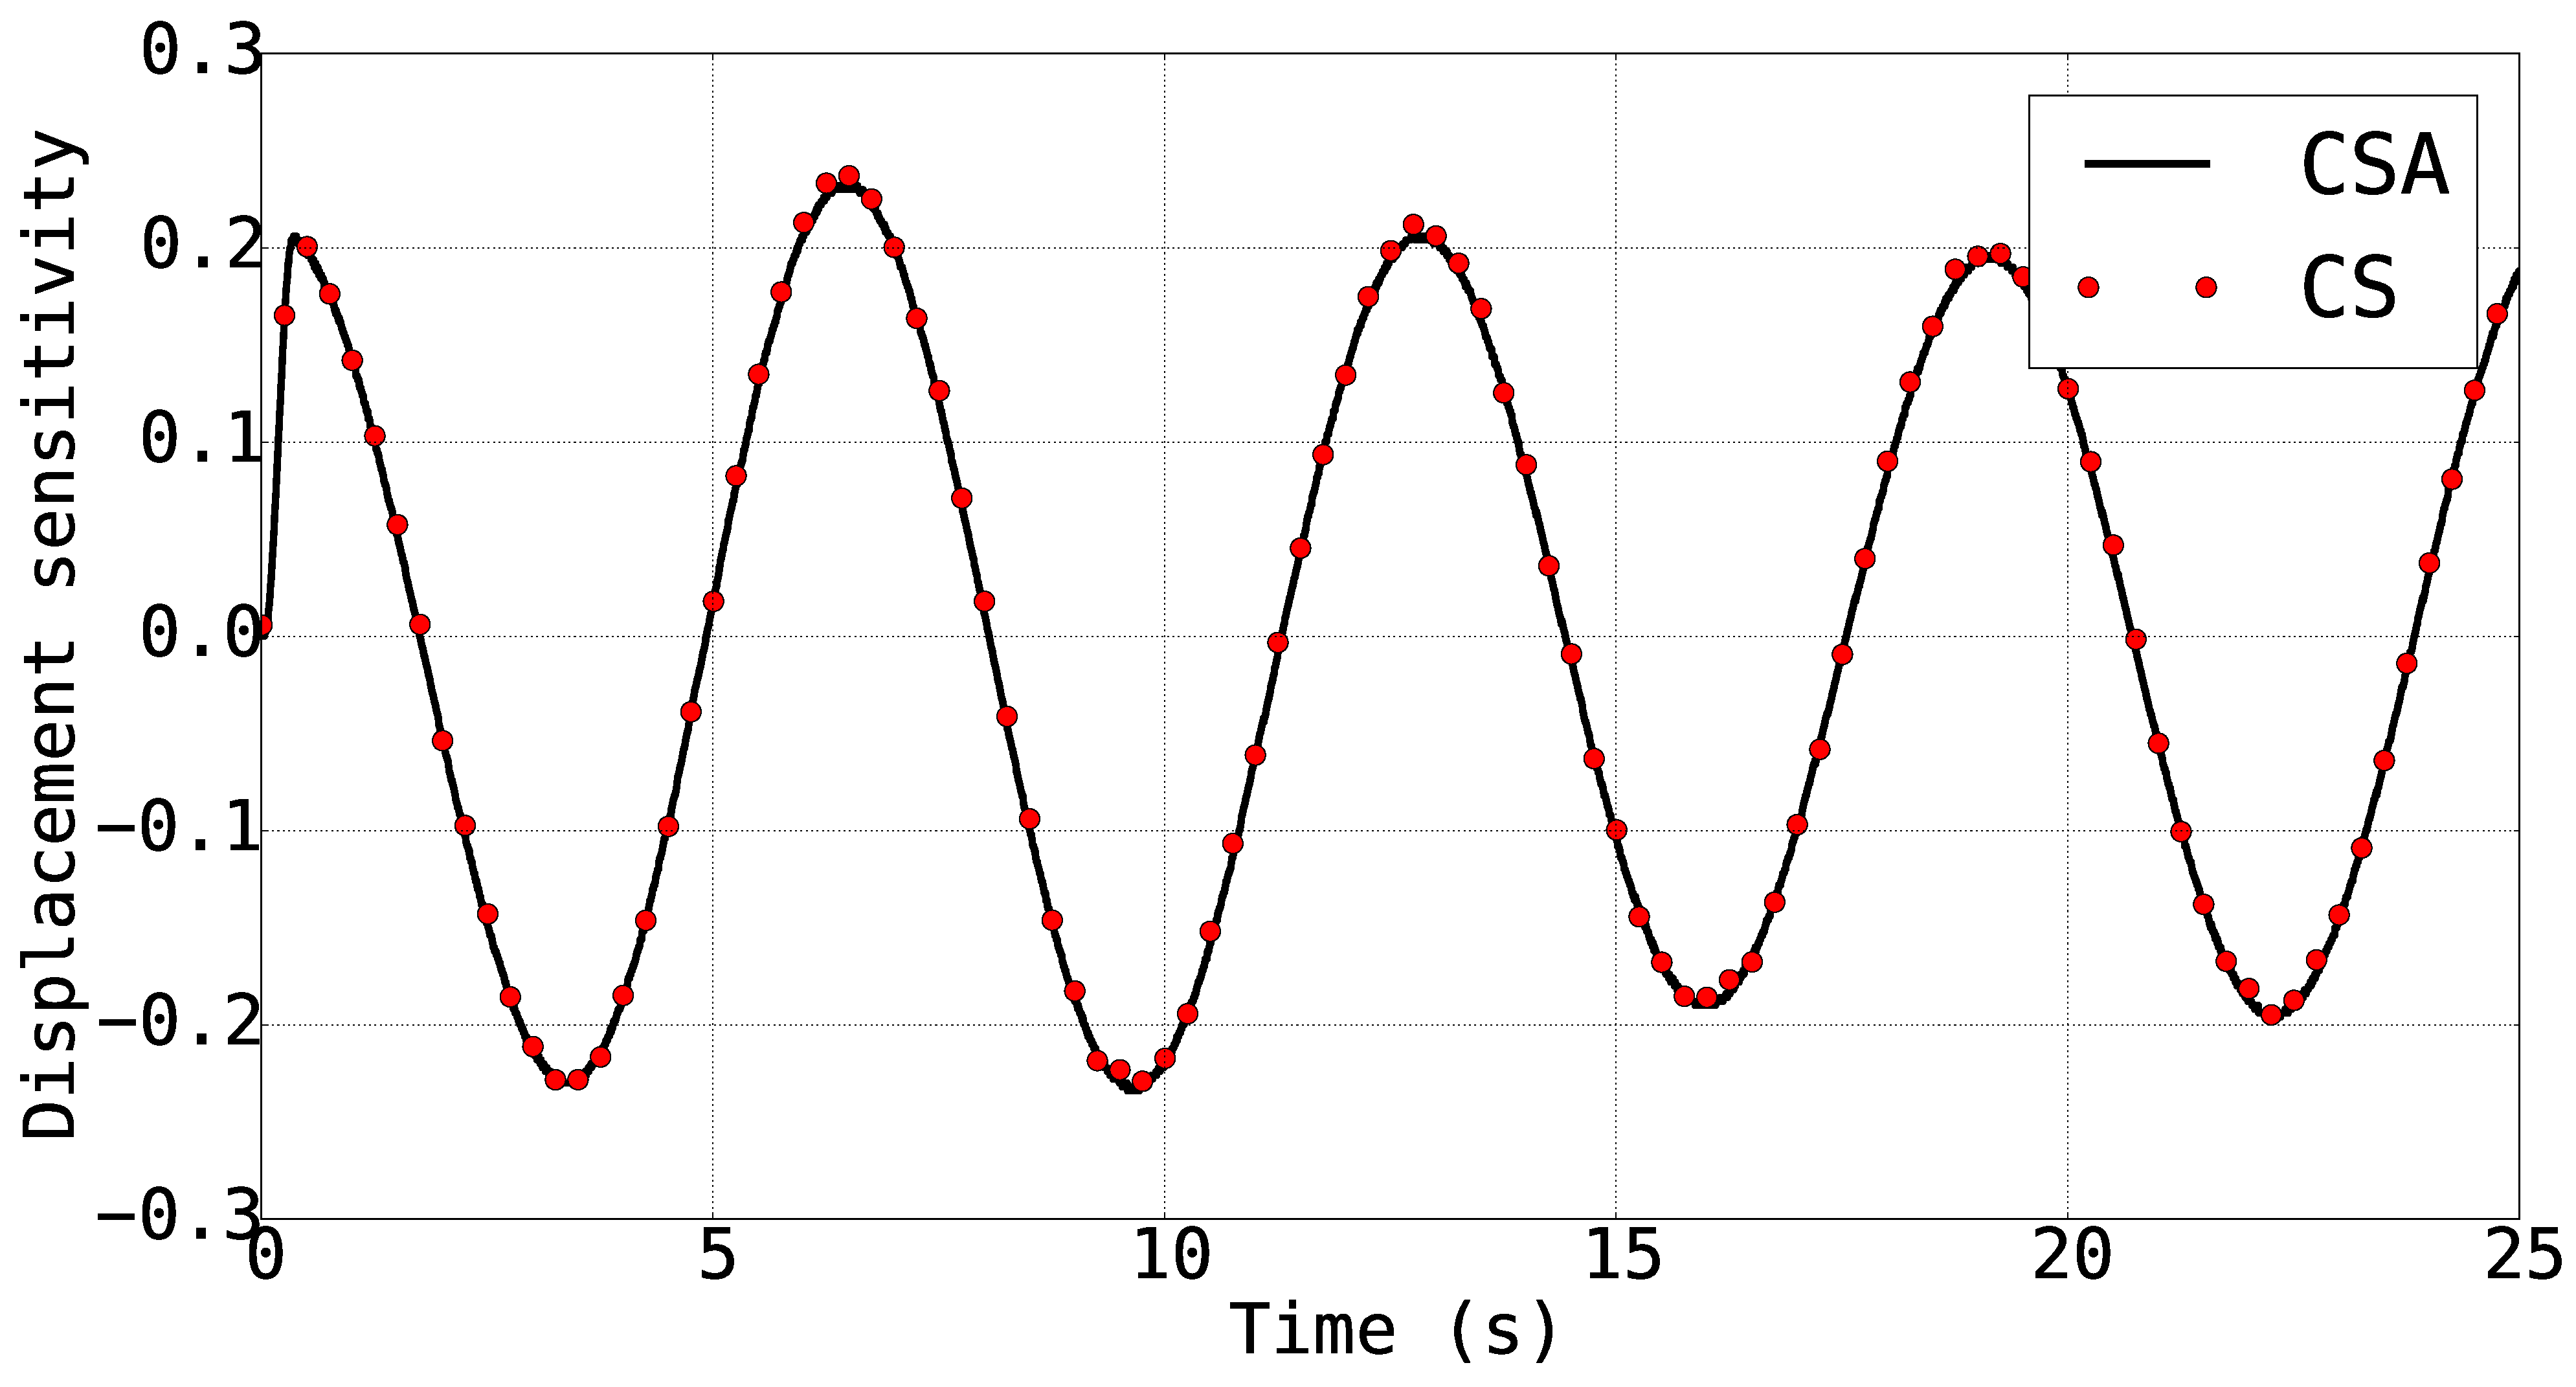
\includegraphics[width=9.0cm]{Chapter_5/figure/cylinder_Re100_DisplacementSensitivity.eps}
    }
    \quad
    \subfigure[$Re = 500$]
    {
    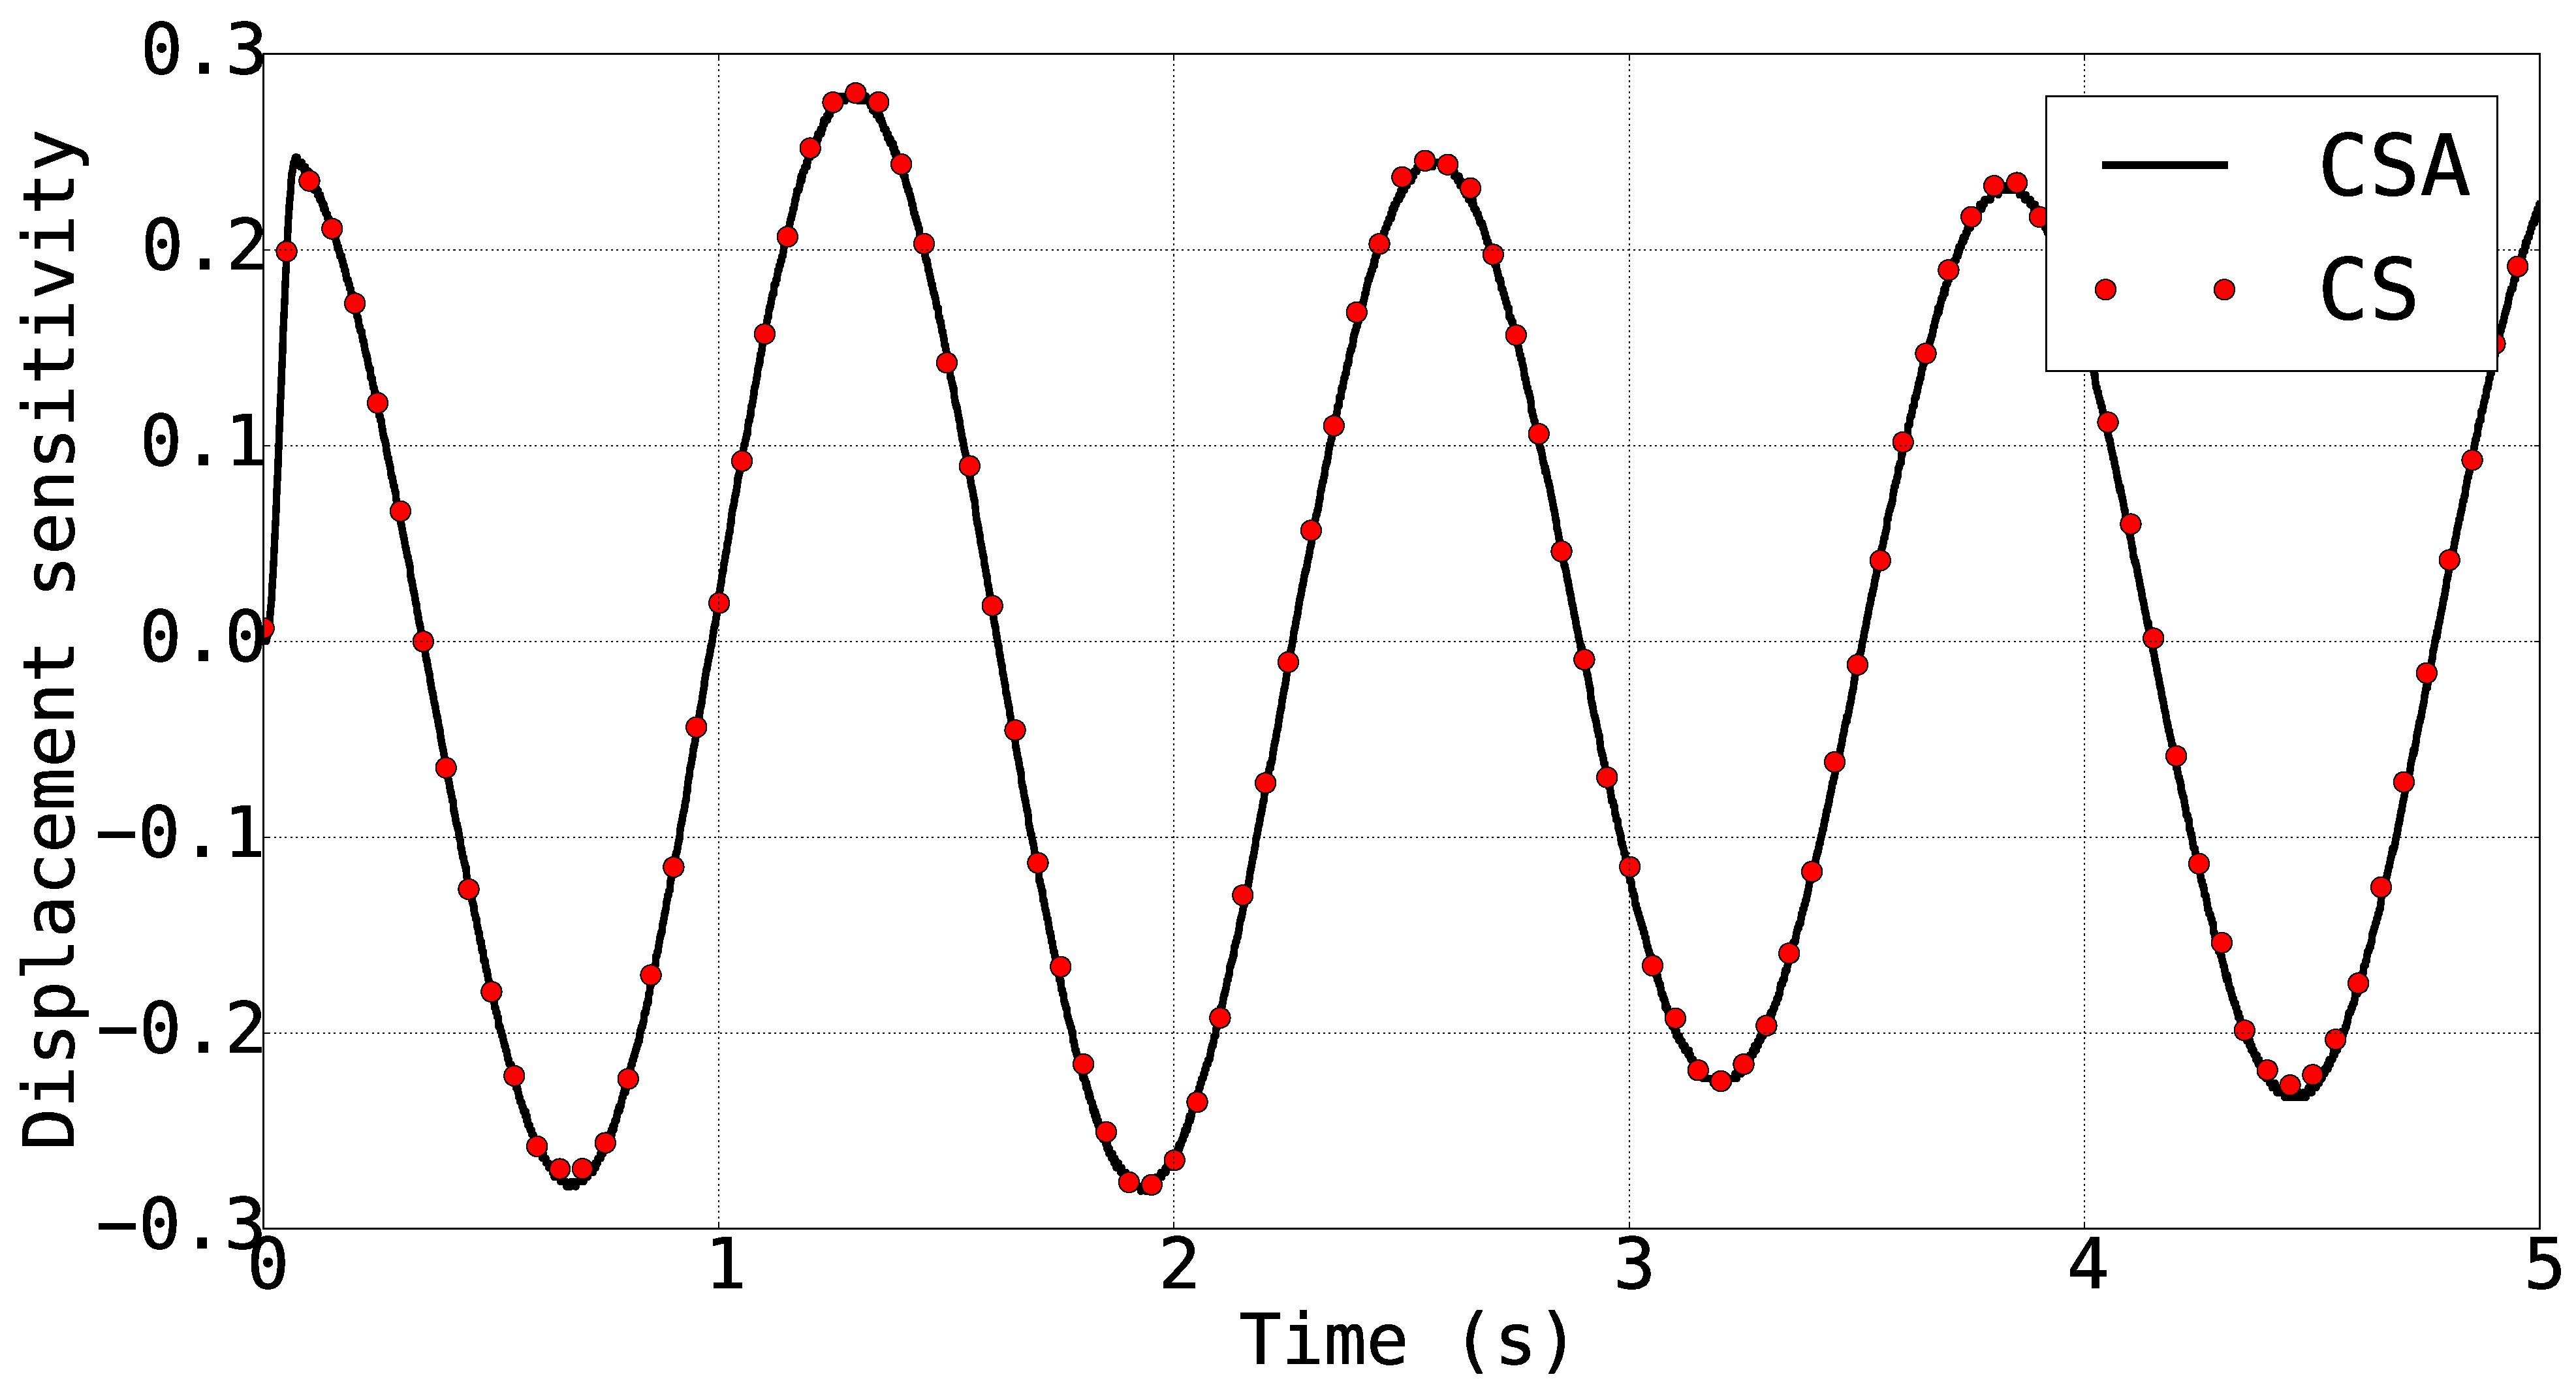
\includegraphics[width=9.0cm]{Chapter_5/figure/cylinder_Re500_DisplacementSensitivity.eps}
    }
    \caption{Time history of cylinder center displacement sensitivity.}
    \label{fig:C5_cylinderDisplacementSensitivity}
\end{figure}
%
Figure \ref{fig:C5_cylinderFSIvelocitySensitivity} shows the u-velocity sensitivity contour around the elastically mounted cylinder at different times. As shown in the sensitivity contours, the change in the cylinder radius mainly affects the downstream flow. This is expected for a convective flow where the information from cylinder cannot move upstream. The small region with negative sensitivity near the surface is due to the reduction of velocity due to boundary layer expansion as the radius increases and has physical meaning.
%
\begin{figure}[H]
    \centering
    \subfigure[$Re = 100, t = 0 \text{ sec}$]
    {
    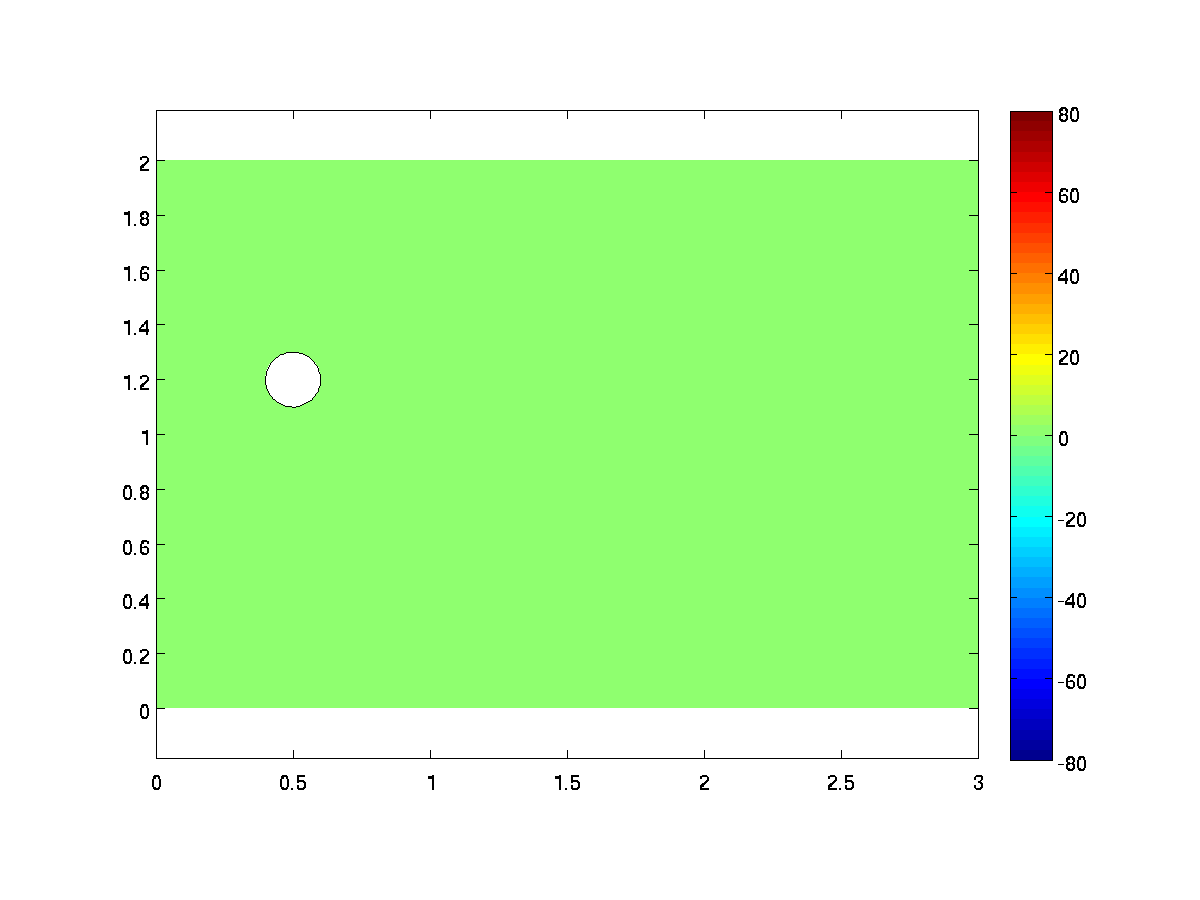
\includegraphics[width=6.0cm]{Chapter_5/figure/cylinder_sensitivity_Re100_t0.png}
    }
    \quad
    \subfigure[$Re = 500, t = 0 \text{ sec}$]
    {
    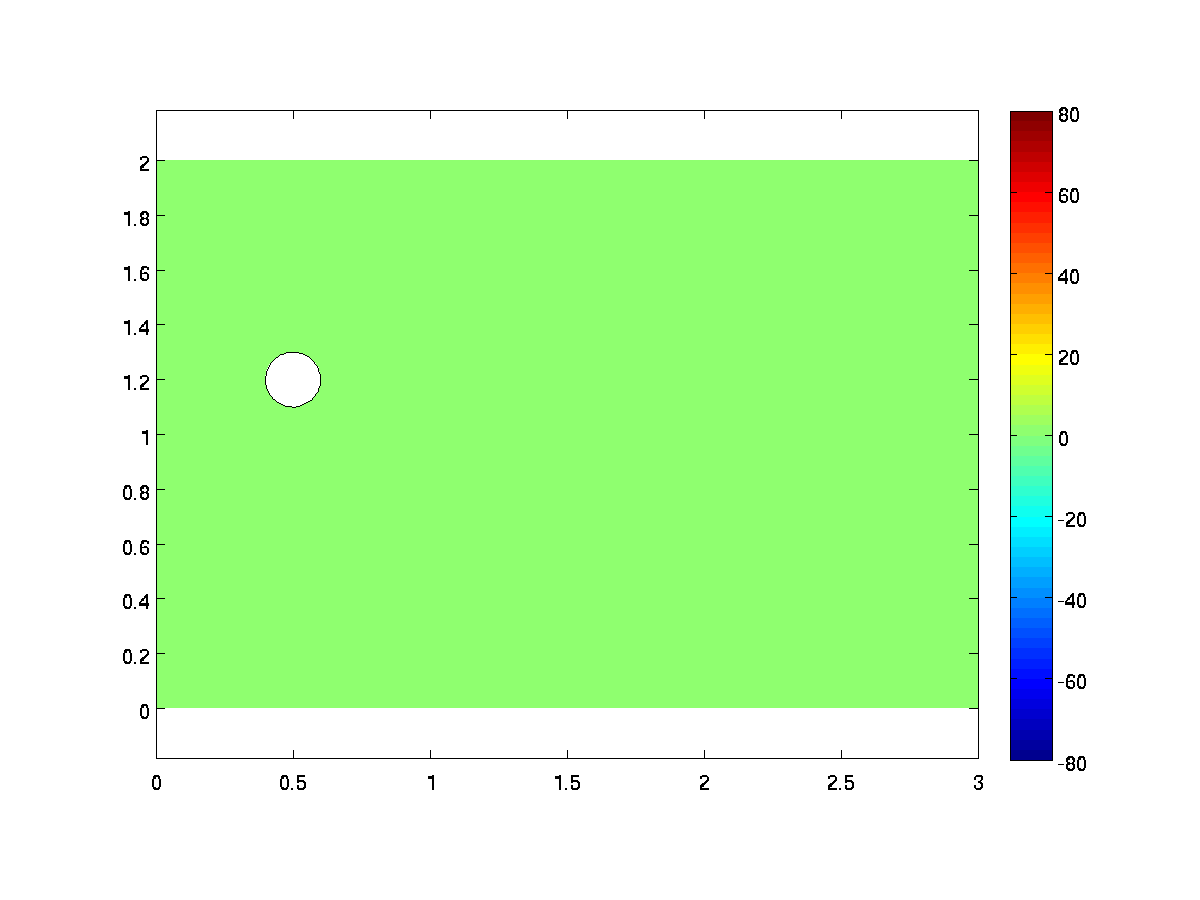
\includegraphics[width=6.0cm]{Chapter_5/figure/cylinder_sensitivity_Re500_t0.png}
    }
    \\
    \subfigure[$Re = 100, t = 0.5 \text{ ec}$]
    {
    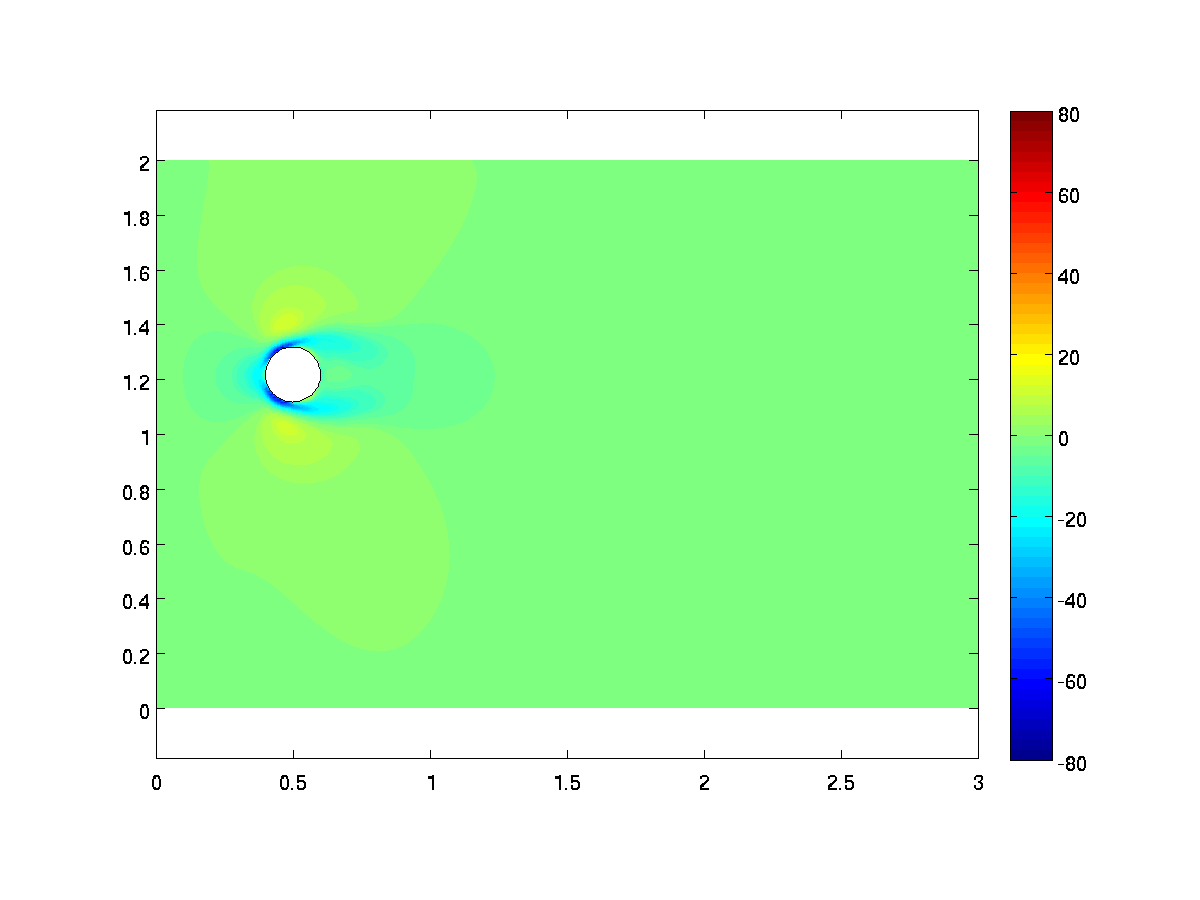
\includegraphics[width=6.0cm]{Chapter_5/figure/cylinder_sensitivity_Re100_t05.png}
    }
    \quad
    \subfigure[$Re = 500, t = 0.5 \text{ sec}$]
    {
    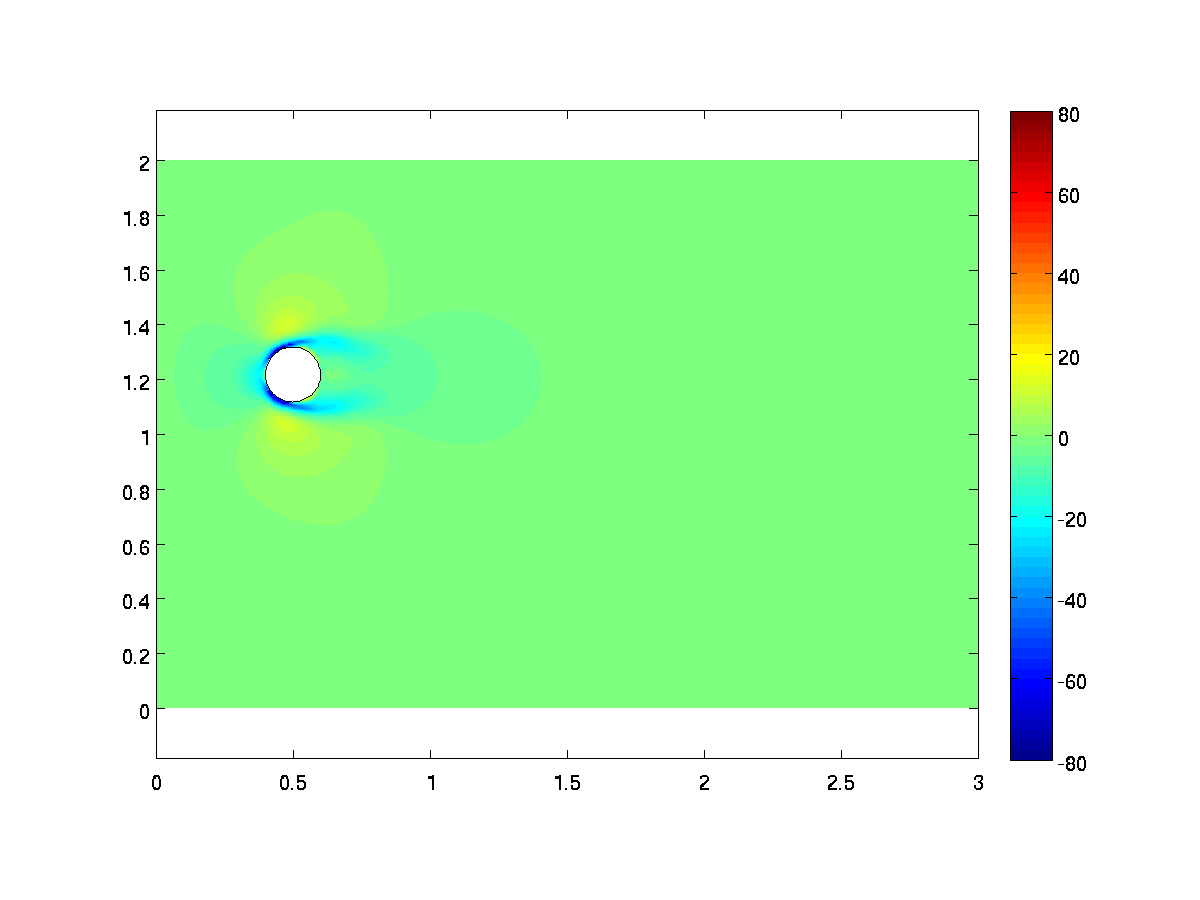
\includegraphics[width=6.0cm]{Chapter_5/figure/cylinder_sensitivity_Re500_t05.png}
    }
    \\
    \subfigure[$Re = 100, t = 5 \text{ sec}$]
    {
    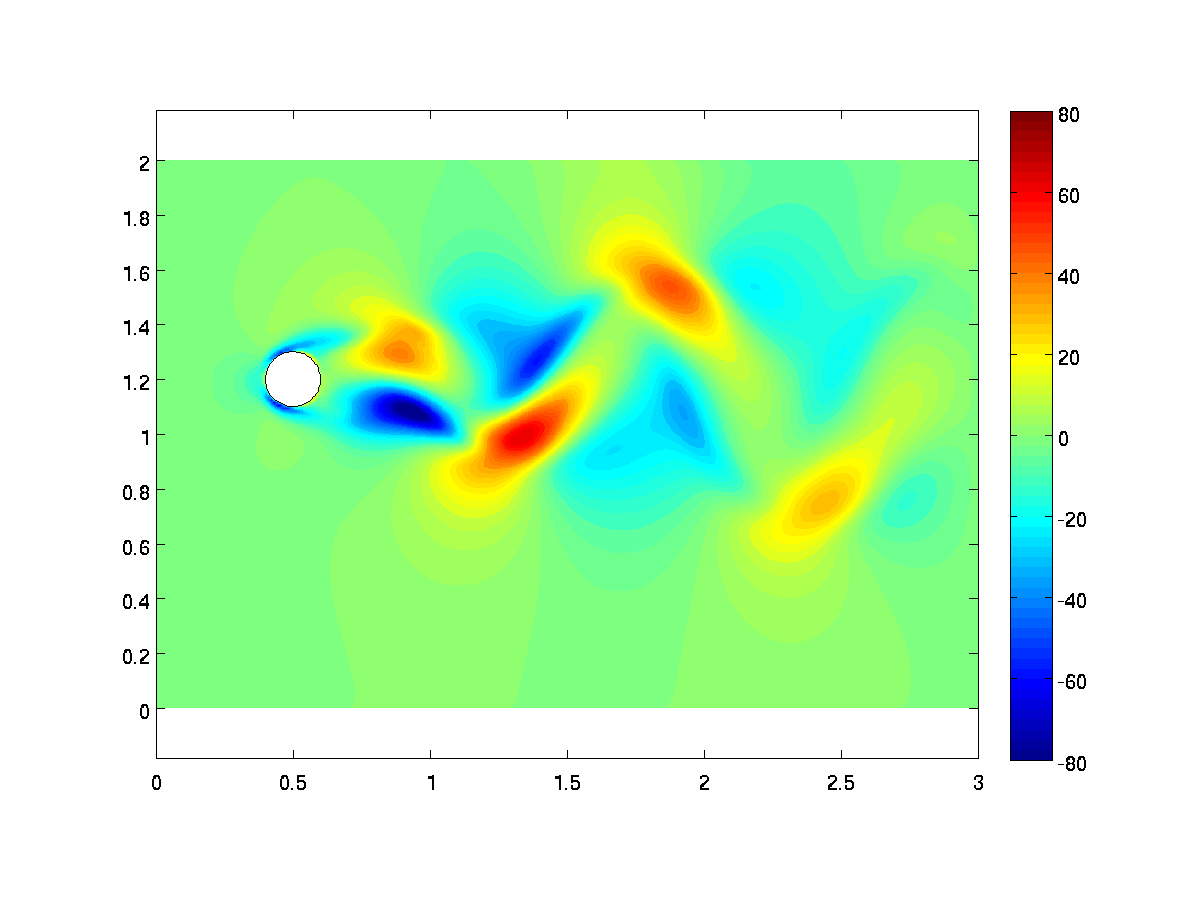
\includegraphics[width=6.0cm]{Chapter_5/figure/cylinder_sensitivity_Re100_t5.png}
    }
    \quad
    \subfigure[$Re = 500, t = 5 \text{ sec}$]
    {
    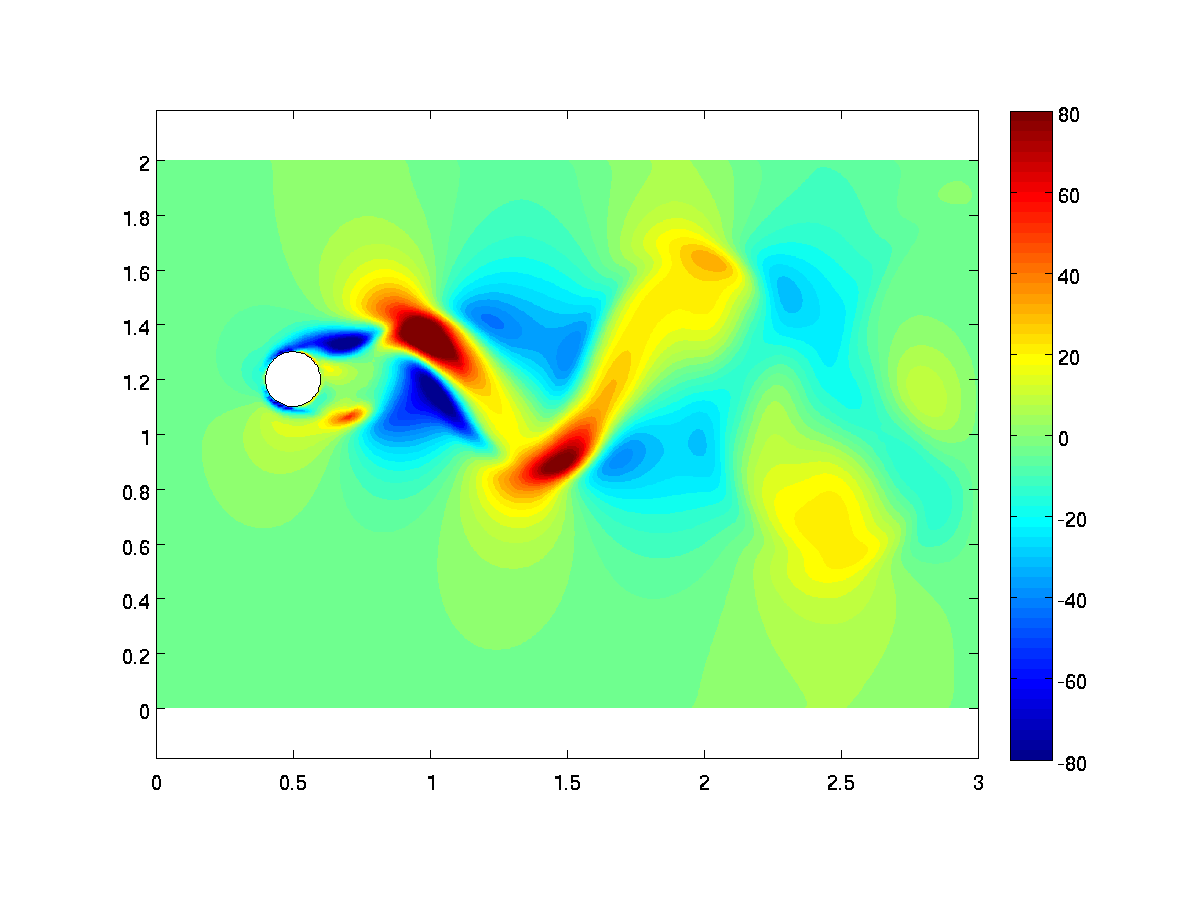
\includegraphics[width=6.0cm]{Chapter_5/figure/cylinder_sensitivity_Re500_t5.png}
    }
    \caption{Unsteady u-velocity contours for flow around cylinder at $Re = 100$ and $Re = 500$.}
    \label{fig:C5_cylinderFSIvelocitySensitivity}
\end{figure}
%